\chapter{心血管系统疾病}

\chapterabstract{本章主要介绍动脉粥样硬化、冠状动脉硬化性心脏病、原发性高血压、风湿病、慢性心瓣膜病、感染性心内膜炎、心肌炎及心肌病。要求掌握动脉粥样硬化的基本病变和复合性病变;冠心病的概念、病因,心绞痛的概念,心肌梗死大体形态特点及对机体的影响;良、恶性高血压病的病变及对机体的影响;风湿病的基本病变,风湿性心脏病的病变及后果;慢性心瓣膜病的发生、病变及血流动力学改变。熟悉重要器官的动脉粥样硬化及对机体的影响;心肌梗死的并发症;三种心内膜炎的区别;心肌炎和心肌病的类型及病变。了解动脉粥样硬化、高血压病和风湿病的病因及发病机制;冠状动脉性猝死;心脏外风湿病变。}

心血管系统包括心脏、动脉、毛细血管和静脉,为一封闭的分支管道系统。血液在此管道系统中朝一定方向不断循环,将氧、各种营养物质、酶和激素等提供给全身各组织,同时,又将组织代谢废物运走。正常的血液循环是保证机体新陈代谢正常进行和体内、外环境动态平衡的重要条件之一。心脏和血管的形态结构发生变化,常可导致功能改变,引起全身或局部血液循环障碍,甚至危及生命。

在欧美等一些发达国家,心血管疾病的死亡率高居总死亡率的第一位。2004年世界心脏联合会宣布,目前全世界每死亡3个人,其中就有1人死于心血管疾病,我国每年死于心血管疾病者在200万人以上,可见心血管疾病对人类健康和生命的威胁之大。因此,心血管疾病受到全世界的广泛关注
。本章主要介绍常见而重要的心脏和动脉疾病。

\section{动脉粥样硬化}
\begin{framed}
    {案例6-1}

    有一病人近年来劳累时,心前区经常疼痛,并向左肩部放射,因病情不缓解,住院治疗。心电图显示系统性心肌缺血,入院后逐渐加重,出现肝大,下肢水肿,在治疗过程中,夜间突然死亡。

    {【问题】}

    (1)该患者死亡原因最可能是什么?

    (2)试分析心脏可能出现的病理变化。
\end{framed}

动脉硬化(arteriosclerosis)是一组以动脉壁增厚、变硬和弹性减退为特征的动脉疾病,包括三种类型:①动脉粥样硬化;②细动脉硬化;③动脉中层钙化。

动脉粥样硬化(atherosclerosis,AS)是最常见的心血管疾病,临床上多见于中、老年人。病变主要累及大、中动脉,以动脉内膜脂质沉积、纤维化和粥样斑块形成为特征,致管壁变硬、管腔狭窄。本病的重要性在于常导致心、脑等重要器官的缺血性病变,严重危害人类健康。

\subsection{病因和发病机制}

\subsubsection{危险因素}

动脉粥样硬化的病因仍不清楚,下列因素被视为危险因素。

\paragraph{高脂血症}
是动脉粥样硬化的主要危险因素。动脉粥样硬化症好发于高脂血症患者,病灶中沉积的主要成分是胆固醇和胆固醇酯。近年来,大量研究结果证明,血浆低密度脂蛋白(LDL)、极低密度脂蛋白(VLDL)水平持续升高与动脉粥样硬化的发病率呈正相关。高密度脂蛋白(HDL)具有很强的抗动脉粥样硬化的作用。

\paragraph{高血压}
高血压病人的动脉粥样硬化发病较早,病变较重。高血压时血流对血管的冲击力较高,可引起内皮细胞损伤和(或)功能障碍,从而导致脂蛋白渗入内膜、单核细胞黏附并迁入内膜、血小板黏附以及动脉中膜平滑肌细胞迁入内膜等一系列变化,促进动脉粥样硬化发生。

\paragraph{吸烟}
过量吸烟可使血液中LDL易于氧化,并导致血液中一氧化碳浓度升高,从而损伤血管内皮细胞;吸烟可使血小板聚集能力增强;烟内含有的某些糖蛋白可激活Ⅻ因子及某些致突变物质,后者可引起血管壁平滑肌细胞增生。这些均有助于动脉粥样硬化的发生和发展。

\paragraph{糖尿病和高胰岛素血症}
糖尿病患者血中VLDL和甘油三酯水平明显升高,HDL水平较低,而且高血糖可致LDL氧化,促进血液单核细胞迁入内膜及转变为泡沫细胞;高胰岛素血症可促进动脉壁平滑肌细胞增生。

\paragraph{遗传因素}
高胆固醇血症和冠心病的家族聚集现象提示本病具有遗传倾向。

\paragraph{其他因素}
动脉粥样硬化的发生随年龄的增长而增加;女性在绝经期前的发病率低于同龄组男性;肥胖易患高脂血症、高血压和糖尿病而促发动脉粥样硬化。

\subsubsection{发病机制}

\paragraph{脂源性学说}
认为高脂血症可引起血管内皮细胞损伤和灶状脱落,导致血管通透性升高,血浆脂蛋白进入内膜,继而引起巨噬细胞的清除反应和血管壁平滑肌增生,形成斑块。

\paragraph{损伤应答学说}
各种原因引起损伤的内皮细胞表达黏附分子增加,吸引单核细胞黏附于内皮,并迁移入内皮下间隙,吞噬脂质后形成单核细胞源泡沫细胞,致内膜出现动脉粥样硬化的早期病变(脂纹)。巨噬细胞、内皮细胞和黏附的血小板均可产生生长因子,刺激中膜平滑肌细胞增生并迁入内膜,继而再产生生长因子,导致纤维斑块形成和病变的继续发展。平滑肌细胞经其表面的LDL受体介导而吞噬脂质,形成平滑肌源性泡沫细胞。损伤应答学说实际上也是一种炎症观点。

\paragraph{受体缺失学说}
已有研究证明,机体的细胞含有特殊的LDL受体,其数目依细胞对胆固醇的需要而增减,若LDL受体数目过少,则可导致细胞从循环血中清除LDL减少,从而使血浆LDL升高,进而促进动脉粥样硬化的发生。

\subsection{基本病理变化}

动脉粥样硬化病变主要发生在大动脉和中等动脉内膜,根据病变发展可将其分为以下几个时期:

\subsubsection{脂纹}

脂纹(fatty
streak)是动脉粥样硬化的早期病变。肉眼观:动脉内膜上出现帽针头大小斑点及宽1~2
mm、长短不一的、与动脉长轴平行的黄色条纹,常位于大、中动脉的血管转弯处或分支开口附近,不隆起或稍隆起于内膜表面。光镜下:病灶处内膜下有大量泡沫细胞聚集。现已证明,泡沫细胞有两种主要来源:一是血管内单核细胞在趋化因子(最重要的是内皮细胞分泌的单核细胞趋化蛋白1)作用下迁入内皮下间隙,被激活成巨噬细胞。该巨噬细胞通过其表面的清道夫受体与氧化的低密度脂蛋白结合并摄取之,继而形成胞浆充满脂质的泡沫细胞(巨噬细胞源性泡沫细胞)。二是在内皮细胞、巨噬细胞、血小板等产生的生长因子(PDGF、FGF、EGF等)作用下,中膜平滑肌细胞增生并迁入内膜,平滑肌细胞表面有LDL受体,可结合、摄取LDL及VLDL而成为泡沫细胞(肌源性泡沫细胞)。脂斑、脂纹的形成和进展见图\ref{fig6-1}和图\ref{fig6-2}A。

\begin{figure}[!htbp]
    \centering
    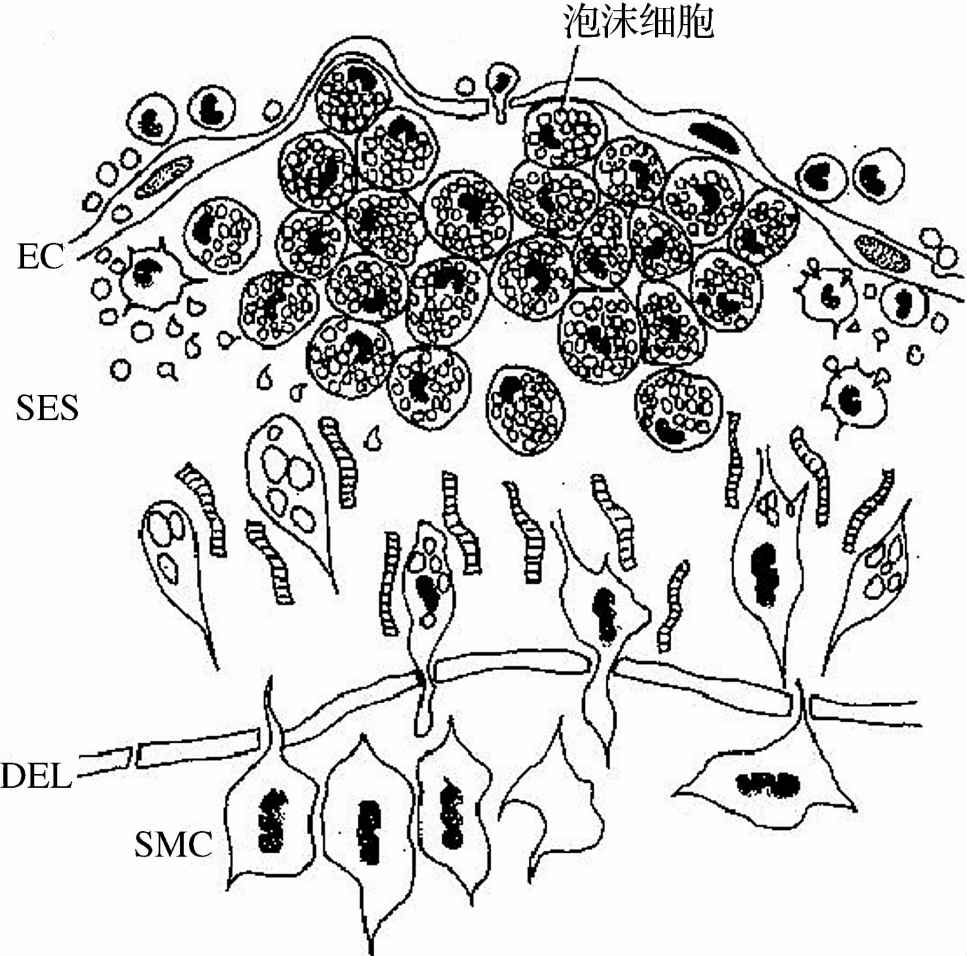
\includegraphics{./images/Image00093.jpg}
    \captionsetup{justification=centering}
    \caption{肌型动脉壁的结构及中膜平滑肌细胞的内移模式图}
    \label{fig6-1}
\end{figure}

\subsubsection{纤维斑块}

脂纹进一步发展则演变为纤维斑块(fibrous
plaque)。肉眼观:纤维斑块为隆起于内膜表面,初为淡黄或灰黄色斑块,随着斑块表层的胶原纤维不断增加及玻璃样变,脂质被埋于深层,斑块逐渐变为灰白色,略带光泽,似蜡滴状(图\ref{fig6-2}A)。光镜下:斑块表面为一层纤维帽,由大量胶原纤维、平滑肌细胞、少数弹力纤维及蛋白聚糖组成。纤维帽下有不等量的泡沫细胞、平滑肌细胞、细胞外基质和炎细胞。纤维斑块的形成是由于氧化的低密度脂蛋白(OX-LDL)的细胞毒性作用,使泡沫细胞坏死,平滑肌细胞大量增生并产生胶原纤维,弹性纤维及蛋白多糖所致。

\subsubsection{粥样斑块}

粥样斑块(atheromatous
plaque)亦称粥瘤,为动脉粥样硬化的典型病变。纤维斑块形成后,在OX-LDL的细胞毒性作用以及内皮细胞及平滑肌细胞产生的氧自由基的作用下,斑块内细胞坏死。泡沫细胞坏死后,释出脂质并释放出许多溶酶体酶,可促进其他细胞坏死崩解。继之,纤维斑块逐渐演变为粥样斑块。肉眼观:为隆起于内膜表面的灰黄色斑块。切面,斑块表层为纤维帽,深部为黄色粥糜样物质。光镜下:纤维帽内胶原纤维发生玻璃样变,深部为大量无定形的坏死崩解物质,其内含有较多细胞外脂质、胆固醇结晶(石蜡切片上为针状空隙),钙盐,其底部和边缘可见肉芽组织增生,外周有少量泡沫细胞和淋巴细胞浸润,中膜因斑块压迫、平滑肌细胞萎缩和弹力纤维破坏而变薄。

\subsubsection{粥样斑块的继发病变}

\paragraph{斑块内出血}
斑块边缘和底部有许多薄壁的新生血管,常易破裂出血(图\ref{fig6-2}B),或因斑块纤维帽破裂血液流入斑块,形成斑块内血肿,使斑块迅速增大,可导致管腔急性阻塞。

\paragraph{斑块破裂}
斑块表层的纤维帽破裂,粥样物质进入血流,可造成胆固醇栓塞,破裂处形成粥样溃疡(图\ref{fig6-2}B)。

\paragraph{血栓形成}
常发生于斑块溃疡处,可造成动脉阻塞,导致器官梗死(如脑梗死、心肌梗死)。血栓可以机化,也可以脱落引起栓塞。

\paragraph{动脉瘤形成}
在病变较严重的动脉壁,由于中膜平滑肌细胞萎缩而变薄,在血管内血压的作用下局部扩张膨出,形成动脉瘤。动脉瘤破裂可发生致命性大出血。

\paragraph{钙化}
钙盐沉积于纤维帽和粥样灶,致动脉壁变硬、变脆,易于破裂。

\begin{figure}[!htbp]
    \centering
    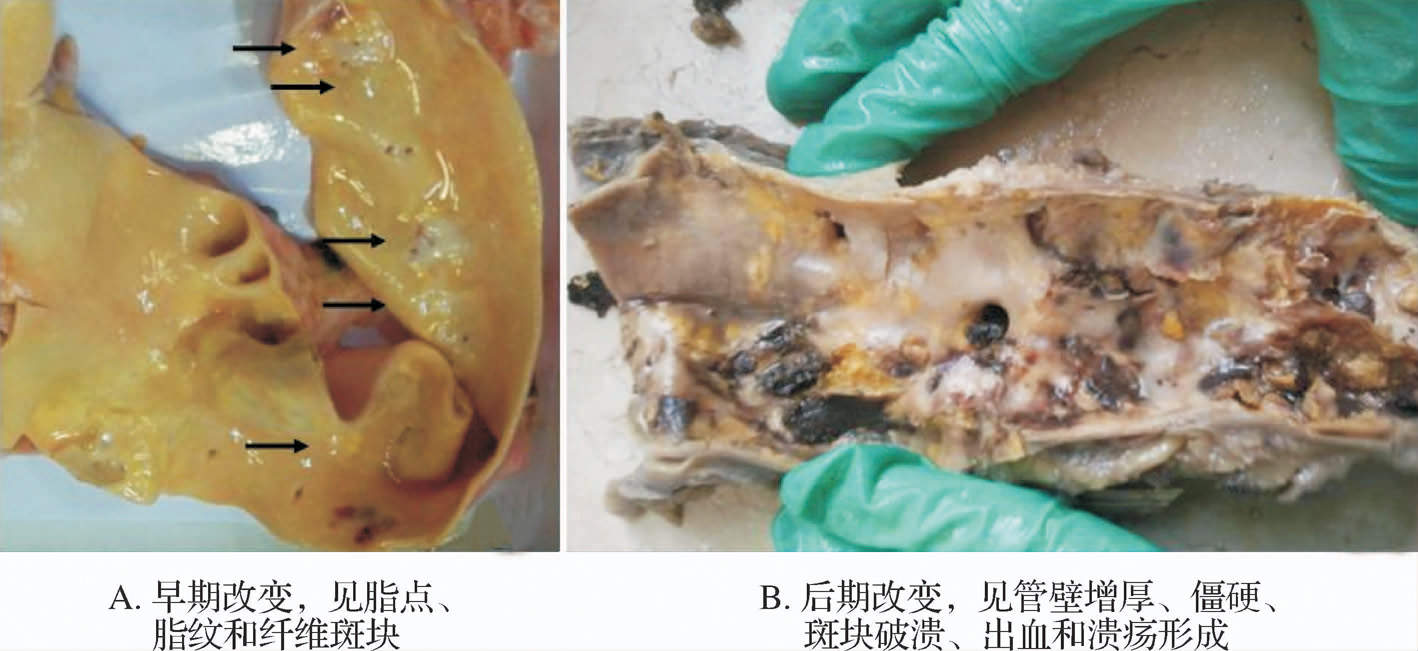
\includegraphics{./images/Image00094.jpg}
    \captionsetup{justification=centering}
    \caption{主动脉粥样硬化}
    \label{fig6-2}
\end{figure}

\subsection{重要器官的动脉粥样硬化症}

\subsubsection{主动脉粥样硬化}

病变多见于主动脉后壁及其分支开口处。以腹主动脉最重,胸主动脉次之,升主动脉最轻。前述的各种动脉粥样硬化的基本病变均可见到。由于主动脉血管口径大,病变一般不引起血流阻塞。病变严重者可形成主动脉瘤,偶见血管破裂。有时形成夹层动脉瘤。

\subsubsection{冠状动脉粥样硬化(详见第二节)}

\subsubsection{脑动脉粥样硬化}

脑动脉粥样硬化的病变以大脑中动脉和willis环最显著。病变血管节段性增粗,管壁变硬,内膜不规则增厚,管腔狭窄甚至闭塞。脑动脉病变使脑组织长期供血不足而逐渐发生萎缩,严重者可有智力减退,甚至痴呆。若脑动脉管腔高度狭窄,继发血栓形成而导致管腔阻塞,可发生脑软化(脑梗死)。严重的脑软化可引起病人失语、偏瘫,甚至死亡。脑动脉粥样硬化病变可形成小动脉瘤,当血压突然升高时可发生致命性的破裂出血。

\subsubsection{肾动脉粥样硬化}

临床并不多见。好发于肾动脉开口处、叶间动脉和弓形动脉。侵犯一侧或两侧肾脏,两肾病变可不对称。病变的动脉管腔狭窄或阻塞,可引起肾缺血、萎缩,间质纤维组织增生和局灶性梗死。梗死机化后形成单个或多个宽大的凹陷性瘢痕。瘢痕较多时,肾体积缩小,称为动脉粥样硬化性固缩肾。

\subsubsection{四肢动脉粥样硬化}

以下肢动脉比较常见且较严重。当较大的动脉管腔明显狭窄时,下肢可因缺血而萎缩、无力,行走时出现间歇性跛行症状。若管腔高度狭窄,闭塞或继发血栓形成,则下肢可因血流中断而发生坏死,甚至坏疽。

\section{冠状动脉粥样硬化性心脏病}

冠状动脉粥样硬化性心脏病(coronary atherosclerotic heart
disease),简称冠状动脉性心脏病(coronary heart
disease,CHD)或冠心病,是指由于冠状动脉粥样硬化,导致心肌缺血、缺氧而引起的心脏病,故又称缺血性心脏病(ischemic
heart
disease,IHD)。广义的冠心病除冠状动脉粥样硬化外,炎症、痉挛、栓塞等冠状动脉病变也可引起急性或慢性缺血性心脏病,但绝大多数冠心病(95%~99%)是由冠状动脉粥样硬化所引起。

\subsection{一、冠状动脉粥样硬化症(coronary
    atherosclerosis)}

冠状动脉粥样硬化最常见于冠状动脉的左前降支,其次为右主干,再次为左主干或左旋支、后降支。病变常呈多发性、节段性分布,一般较大分支病变较重。由于血流冲击的缘故,通常靠近心肌一侧的动脉壁病变更为严重。在横切面上斑块多呈半月形,管腔发生不同程度的狭窄(图\ref{fig6-3})。根据斑块引起管腔狭窄的程度,可将其分为四级:Ⅰ级,管腔狭窄在25%以下;Ⅱ级,狭窄在26%~50%;Ⅲ级,狭窄在51%~75%;Ⅳ级,管腔狭窄在76%以上。

\begin{figure}[!htbp]
    \centering
    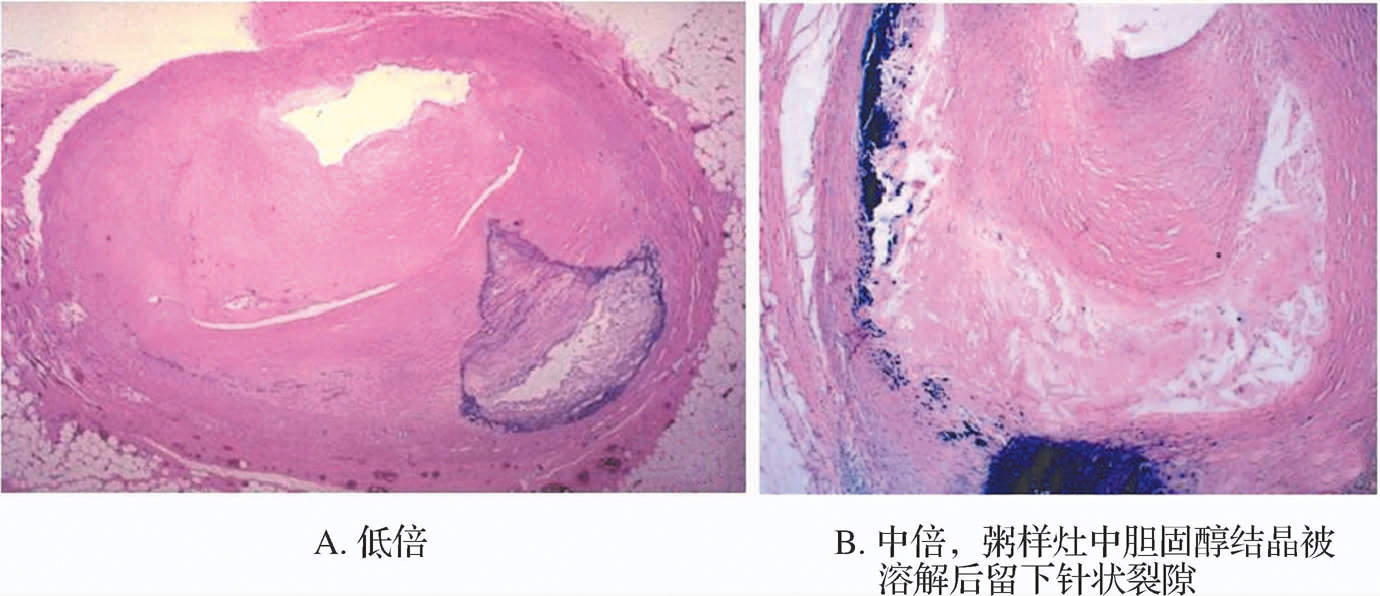
\includegraphics{./images/Image00095.jpg}
    \captionsetup{justification=centering}
    \caption{冠状动脉粥样硬化,IV级(HE染色)\\{\small 冠状动脉内膜下层有粥瘤形成,致管腔狭窄,图中灰蓝色颗粒为钙盐沉积}}
    \label{fig6-3}
\end{figure}



\subsection{冠状动脉粥样硬化性心脏病}

根据心肌缺血的轻重和缓急,心肌损伤的程度以及侧支循环建立等情况,冠心病在临床上可表现为心绞痛、心肌梗死、心肌硬化和冠状动脉性猝死。

\subsubsection{心绞痛}

心绞痛(angina
pectoris)是由于心肌急性、暂时性缺血缺氧所造成的以胸骨后疼痛为特点的临床综合征。表现为阵发性胸骨后、心前区疼痛或紧迫感,疼痛常放射到左肩和左臂。一般认为,心绞痛的发生是在冠状动脉粥样硬化基础上,由于体力活动、情绪激动、寒冷、暴饮暴食等因素引起冠状动脉痉挛,心肌缺血缺氧,酸性代谢产物堆积刺激感觉神经末梢所产生的反射性症状。心绞痛一般历时短暂,发作后心肌的代谢和功能可恢复正常。但如反复发作,心肌也可发生灶状坏死。

\subsubsection{心肌梗死}

心肌梗死(myocardial
infarction,MI)是由于严重而持续的缺血缺氧所引起的较大范围的心肌坏死。

\paragraph{原因}
①冠状动脉粥样硬化并发血栓形成。②冠状动脉持续痉挛。③在冠状动脉粥样硬化基础上,心脏过度负荷。上述原因均可导致心肌供血不足,甚至阻断,引起心肌梗死。

\paragraph{好发部位和范围}
心肌梗死的部位和范围与病变血管的供血区域一致。心肌梗死多发生于左心室,其中左心室前壁、心尖部及室间隔前2/3约占全部心肌梗死的50%,该区正是左前降支供血区;约25%的心肌梗死发生在左心室后壁、室间隔后1/3及右心室(图\ref{fig6-4});左心室侧壁梗死较少见。

\begin{figure}[!htbp]
    \centering
    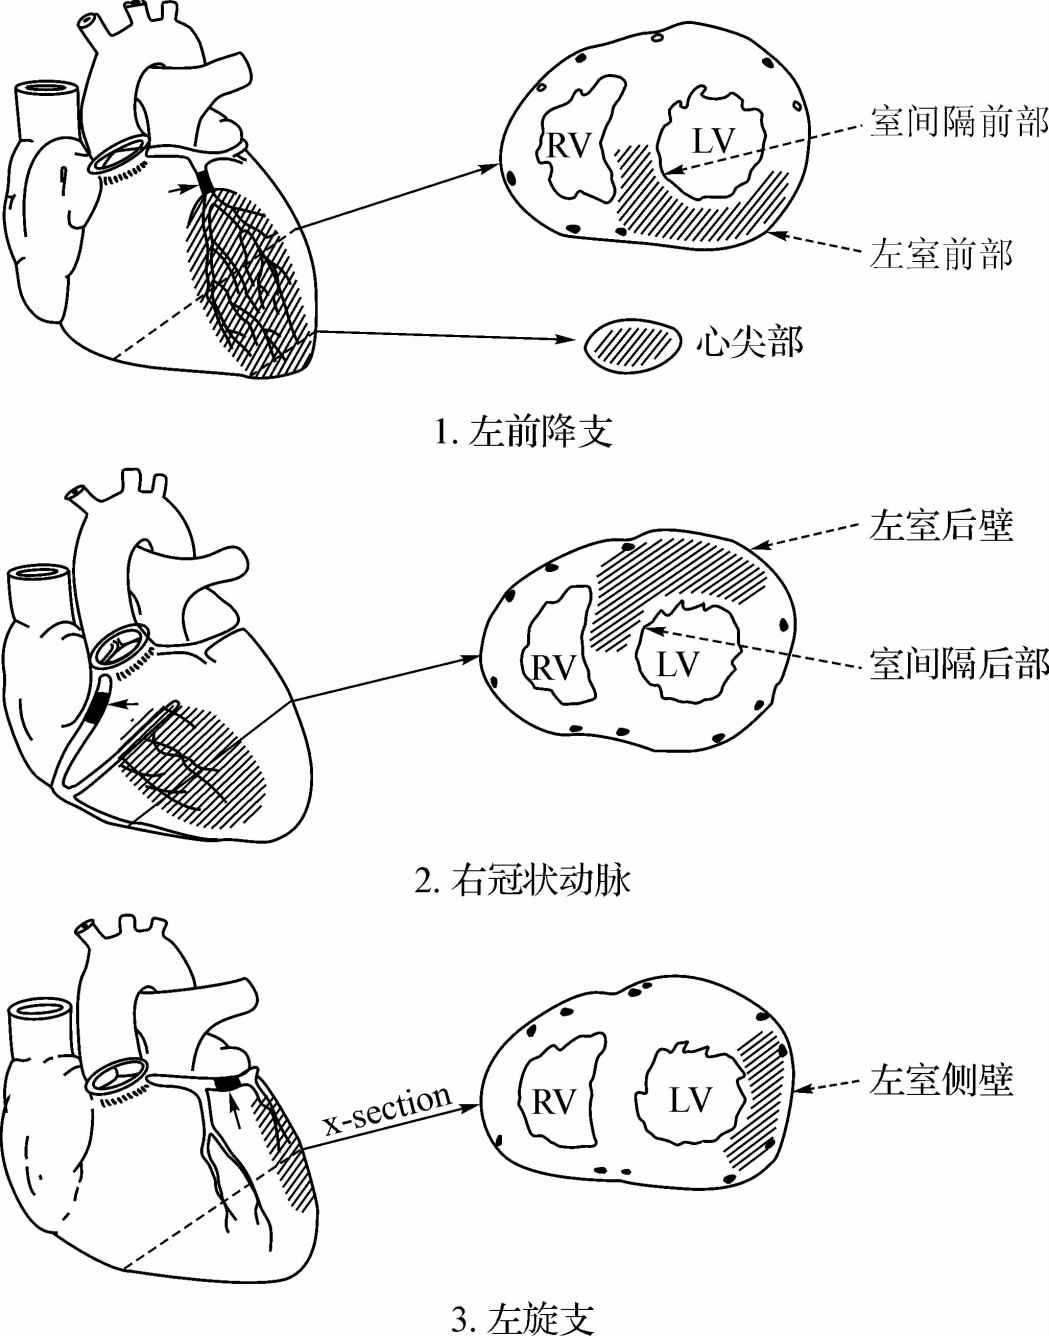
\includegraphics{./images/Image00096.jpg}
    \captionsetup{justification=centering}
    \caption{冠状动脉粥样硬化好发部位及心肌梗死常见部位}
    \label{fig6-4}
\end{figure}

大多数心肌梗死累及心室壁全层,称为透壁性心肌梗死。少数病例仅累及心室壁内侧1/3的心肌(可波及肉柱和乳头肌),称为心内膜下心肌梗死。

\paragraph{病理变化}
心肌梗死属于贫血性梗死,形态表现与患者发病后存活的时间有关。一般在梗死6小时后肉眼才能辨认。肉眼观:6小时后梗死心肌呈苍白色,梗死灶形状不规则,8~9小时呈土黄色,较干燥,失去光泽,4天后梗死灶呈灰白色,周边出现充血出血带。2~3周后由于肉芽组织取代之而呈红色,5周后逐渐形成瘢痕而呈灰白色,质较硬。光镜下:心肌梗死属凝固性坏死,梗死灶内心肌细胞变性、坏死,肌原纤维及细胞核溶解消失。梗死灶边缘可见充血、出血及中性粒细胞浸润(图\ref{fig6-5})。2~3周后梗死灶内见肉芽组织,5周后变成瘢痕组织。

\begin{figure}[!htbp]
    \centering
    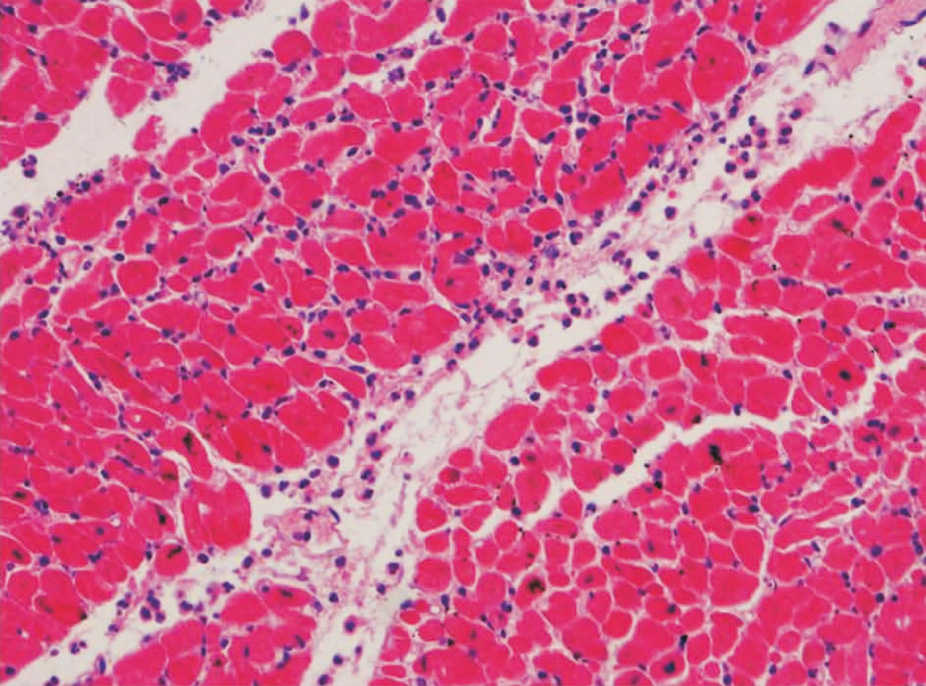
\includegraphics{./images/Image00097.jpg}
    \captionsetup{justification=centering}
    \caption{急性心肌梗死(HE染色,中倍)}
    \label{fig6-5}
\end{figure}

\paragraph{心肌梗死的生化改变}
心肌梗死1小时后细胞膜的通透性增高,钠和钙离子移入,钾离子溢出。2~3小时后,细胞内部的各种酶活性逐渐降低直至消失,而血清中的某些酶浓度先后增高,以后下降再恢复正常,如肌酸磷酸激酶(CPK)、谷氨酸-草酰乙酸转氨酶(门冬氨酸氨基转移酶,AST)及乳酸脱氢酶(LDH)等。故在一定时间内检查血清酶活性有助于对心肌梗死的诊断,尤以CPK意义最大。由于心肌缺血早期可引起心肌细胞肌红蛋白丢失,释放入血并经尿液排出,因此急性心肌梗死病人较早地出现血液和尿液中肌红蛋白增高。

\paragraph{并发症及后果}
心肌梗死,尤其是透壁性梗死,可合并下列并发症(图\ref{fig6-6})。

(1)心脏破裂:较少见,多发生于心肌梗死后1~2周内,主要由于梗死灶及周围中性白细胞释出蛋白水解酶,使梗死灶心肌软化所致。患者可发生猝死。

(2)室壁瘤:可发生于心肌梗死的急性期,更常见于愈合期。梗死区坏死组织或瘢痕组织在心室内血液压力作用下,局部向外膨出而成。室壁瘤可继发血栓形成或破裂。

(3)附壁血栓形成:由于梗死区心内膜粗糙或室壁瘤处出现涡流等原因,为血栓形成提供了条件。血栓可发生机化,或脱落引起体循环动脉栓塞。

(4)心源性休克:梗死面积大于40%时,心肌收缩力极度减弱,心输出量显著下降,可发生心源性休克。

(5)心肌梗死后综合征:发生于心肌梗死后数周或数月内,表现为心包炎、胸膜炎或肺炎。其发生可能与机体对坏死物质发生过敏反应有关。

(6)心力衰竭:梗死的心肌收缩力显著减弱以至丧失,可导致不同程度的心力衰竭。

(7)心律失常:因传导系统受累及心肌梗死所致的电生理紊乱而引起。

\begin{figure}[!htbp]
    \centering
    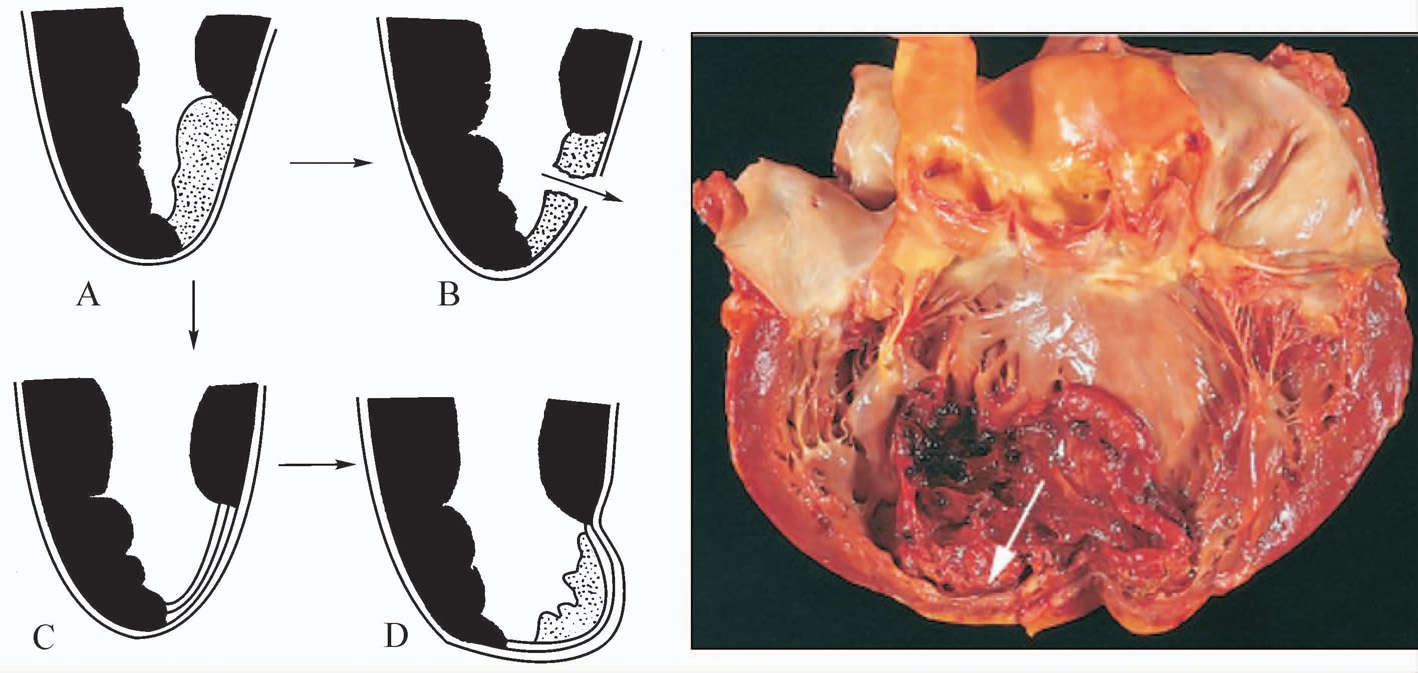
\includegraphics{./images/Image00098.jpg}
    \captionsetup{justification=centering}
    \caption{心肌梗死后果图}
    \label{fig6-6}
\end{figure}

\subsubsection{心肌硬化}

心肌硬化即广泛的心肌纤维化。冠状动脉粥样硬化时,动脉管腔狭窄,心肌长期缺血缺氧,引起心肌萎缩,间质纤维组织增生导致心肌硬化。心肌硬化会导致慢性心功能不全。

\subsubsection{冠状动脉性猝死}

多见于40~50岁患者,男性比女性多3.9倍。可发生于某种诱因后,如饮酒、劳累、吸烟或运动后,患者突然昏倒,四肢抽搐、小便失禁,或突然发生呼吸困难、口吐白沫、迅速昏迷。可立即死亡或在1至数小时后死亡。但有不少病例,死于夜间睡眠中。尸体解剖最常见的是冠状动脉粥样硬化,常有1支以上的冠状动脉呈中至重度狭窄,部分病例有继发病变,如血栓形成或斑块内出血,无其他致死性病变。而有的病例冠状动脉粥样硬化病变较轻,推测与合并冠状动脉痉挛有关。

\section{高血压病}
\begin{framed}
    {案例6-2}

    {【病例摘要】}

    一例无主女尸,剖检发现死者两肾体积缩小,重量减轻各为80
    g,质地硬,皮质变薄,表面呈颗粒状,肾切片观察,均有细动脉透明变性,肾小球纤维化等改变。

    {【问题】}

    (1)此患者生前可能患的疾病是什么?

    (2)此患者其他器官可能有哪些病变?
\end{framed}

成年人收缩压≥140 mmHg(18.6 kPa)和(或)舒张压≥90 mmHg(12
kPa)被定为高血压。高血压(hypertension)可分为原发性高血压(primary
hypertension)和继发性高血压(secondary
hypertension),后者又称为症状性高血压,占5%~10%,由某些疾病引起,高血压是其中症状之一,如慢性肾小球肾炎、肾动脉狭窄和肾上腺肿瘤时,患者的血压可以升高。原发性高血压又称高血压病,占90%~95%,是一种原因未明的、以体循环动脉血压持续性升高为主要临床表现的独立性全身性疾病。本病是一种常见病,病变主要累及全身细小动脉,常引起心、脑、肾等重要脏器病变,并伴有相应的临床表现,严重者可因心力衰竭、脑出血和肾衰竭而死亡。

\subsection{病因和发病机制}

高血压病的病因和发病机制尚未阐明,一般认为是综合因素的作用结果。

\paragraph{遗传因素}
约75%的患者具有遗传素质,同一家族中高血压病患者常集中出现。近年的研究结果显示,某些基因的变异和突变,或遗传缺陷与高血压发生有密切关系,如血管紧张素(AGT)基因缺陷等,通过不同机制引起血压升高。

\paragraph{膳食因素}
膳食中高钠能使血容量增加,血压升高。钾能促进排钠,有可能保护动脉不受钠的不良作用影响。多数人认为膳食低钙是高血压的危险因素,钙可减轻钠的升压作用。

\paragraph{社会心理因素}
据调查,精神长期处于紧张状态的职业,其高血压患病率高。以及遭受应激性生活事件(如父母早亡、失恋、丧偶、家庭成员意外伤亡、家庭破裂、经济和政治冲击等)刺激者高血压患病率比对照组高。据认为,以上因素可改变体内激素平衡,从而影响所有代谢过程。

\paragraph{神经内分泌因素}
一般认为,神经调节功能障碍和细动脉的交感神经纤维兴奋性增强是高血压发病的重要因素。体内的肾上腺素、去甲肾上腺素、肾上腺皮质激素以及前列腺素F2a等多种激素共同参与了高血压的形成。

\subsection{类型和病理变化}

原发性高血压可分为良性高血压病和恶性高血压病两类。病变主要累及全身细小动脉(中膜仅有1~2层平滑肌和血管口径在1
mm以内的动脉),由于细小动脉的病变常引起心、脑、肾及眼底的病变。良性和恶性高血压病的病理变化不同。

\subsubsection{良性高血压病}

良性高血压病(benign
hypertension)又称缓进型高血压病,约占高血压的95%,多发生在中年以后,进展缓慢,早期无明显症状,往往在体检时发现。病变开始表现为全身细小动脉痉挛,血压间断性升高并处于波动状态。此后,血压持续性升高并出现多个脏器的继发病变。晚期可因心、脑病变而死亡,死于肾病变者较少。按病变的发展过程分为三期。

\paragraph{机能紊乱期}
为高血压病早期阶段,全身细小动脉间歇性痉挛收缩,管腔缩小,外周阻力增加,而使血压升高。此期动脉血管本身无器质性病变,痉挛解除后血压可恢复正常。临床上病人血压升高,但常有波动,可伴有头痛头晕症状。经适当的休息和治疗血压可恢复正常。

\paragraph{动脉病变期}
长期的细小动脉痉挛和血压持续升高,逐渐引起细小动脉硬化。

(1)细动脉硬化:细动脉硬化是高血压病最主要的病变特征,表现为细动脉玻璃样变性,见于直径小于0.3
mm中膜仅有1~2层平滑肌细胞的细动脉,如肾小球入球动脉、脾小体的中央动脉及视网膜小动脉等。由于长期细动脉痉挛,管壁缺氧,内皮细胞和基底膜通透性增高,血浆蛋白渗入内皮下间隙,与局部平滑肌细胞在抗损伤过程中产生的修复性胶原纤维及蛋白多糖混合,使细动脉壁玻璃样变,形成细动脉硬化。严重时细动脉壁明显增厚、变硬、管腔狭窄,甚至管腔闭塞。光镜下见细动脉壁增厚、均匀红染无结构,管腔狭窄甚至闭塞(图\ref{fig6-7})。

\begin{figure}[!htbp]
    \centering
    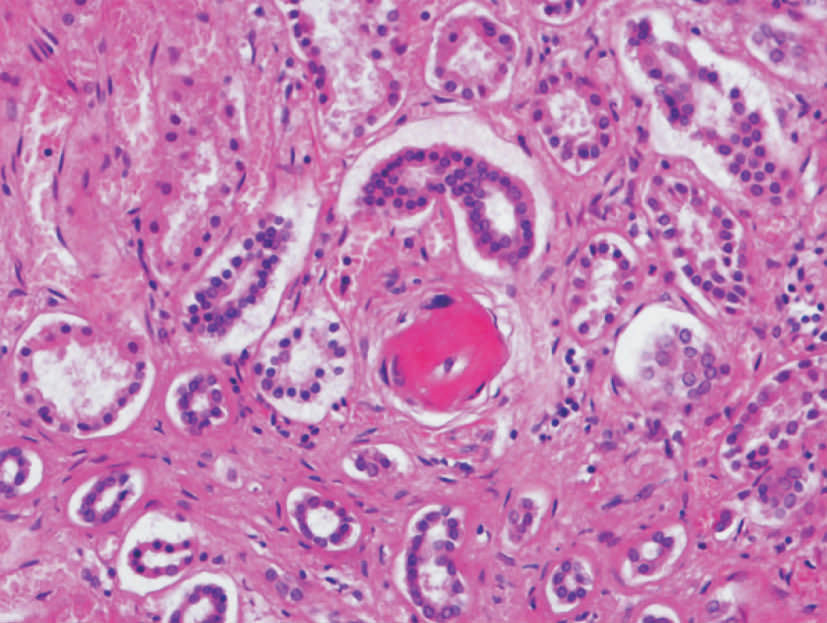
\includegraphics{./images/Image00099.jpg}
    \captionsetup{justification=centering}
    \caption{肾细动脉硬化(HE染色,中倍)\\{\small 图中部可见一细动脉,管腔狭小,管壁增厚僵硬,呈均质红染无结构物}}
    \label{fig6-7}
\end{figure}



(2)小动脉硬化:主要累及肌型小动脉,如肾弓形动脉,小叶间动脉及脑内小动脉。光镜下,肌型小动脉内膜平滑肌细胞、胶原及弹性纤维增生、内弹力膜分裂,分层,致内膜增厚。中膜平滑肌细胞肥大增生,不同程度的胶原纤维、弹性纤维增生,致中膜增厚。上述病变致小动脉壁增厚,变硬,弹性减弱,管腔狭窄。

(3)大动脉硬化:主动脉及主要分支等血管,可伴发动脉粥样硬化或无明显病变。

此期病人血压进一步升高,失去波动性,休息后也不易降为正常。随着细小动脉的硬化,高血压不断加重,内脏发生继发性病变。

\paragraph{内脏病变期}
最重要的是心、脑、肾和视网膜的病变。

(1)心脏:长期高血压引起的心脏病变称为高血压性心脏病(hypertensive
heart
disease),其主要病变是左心室肥大,由于细小动脉硬化,外周阻力增加,左心室负荷增大,久之发生代偿性肥大,此时肉眼观心脏体积增大,重量增加,可达400
g以上(正常250 g左右)甚至可达900~1 000 g。左心室壁肥厚,可达1.5~2.0
cm(正常0.9~1.2
cm),左心室肉柱和乳头肌增粗,心腔不扩张,相对缩小,称为向心性肥大(concentric
hypertrophy)。光镜下见心肌纤维增宽,变长,分支较多,核肥大深染。肥厚的左心室负荷继续增加,超过其代偿能力而逐渐发生代偿失调,心肌收缩力降低,逐渐出现心腔扩张,称为离心性肥大(eccentric
hypertrophy),严重时可发生左心衰竭,出现肺淤血和水肿,患者可感心悸,呼吸困难,发绀,最后可导致右心衰竭而出现全身淤血水肿。

(2)肾脏:表现为原发性颗粒性固缩肾(primary granular atrophy of the
kidney),常为双侧对称性、弥漫性的病变。肉眼观:肾脏体积缩小,重量减轻,质地变硬,表面满布红色细颗粒。切面,肾皮质变薄,一般在0.2
cm左右,皮、髓质分界不清,叶间动脉和弓形动脉管壁增厚,管腔哆开。光镜下:肾细、小动脉硬化,管壁增厚,管腔狭窄。所属肾小球发生纤维化和玻璃样变,相应的肾小管因缺血而萎缩、消失(图\ref{fig6-8});肾间质结缔组织增生,淋巴细胞浸润。病变处肾实质萎缩,结缔组织增生、收缩使肾表面凹陷;病变轻微区的肾单位发生代偿性肥大、扩张,向肾表面凸起。因萎缩与代偿区弥漫性交杂分布,形成肉眼所见的细颗粒状。临床上,病变早期可以不出现明显症状。晚期,由于大量的肾单位受损,肾血流量减少,肾小球滤过率逐渐降低而出现肾功能不全。患者可出现蛋白尿、管型尿和肾功能障碍的表现。严重者可以出现尿毒症,甚至导致死亡。

\begin{figure}[!htbp]
    \centering
    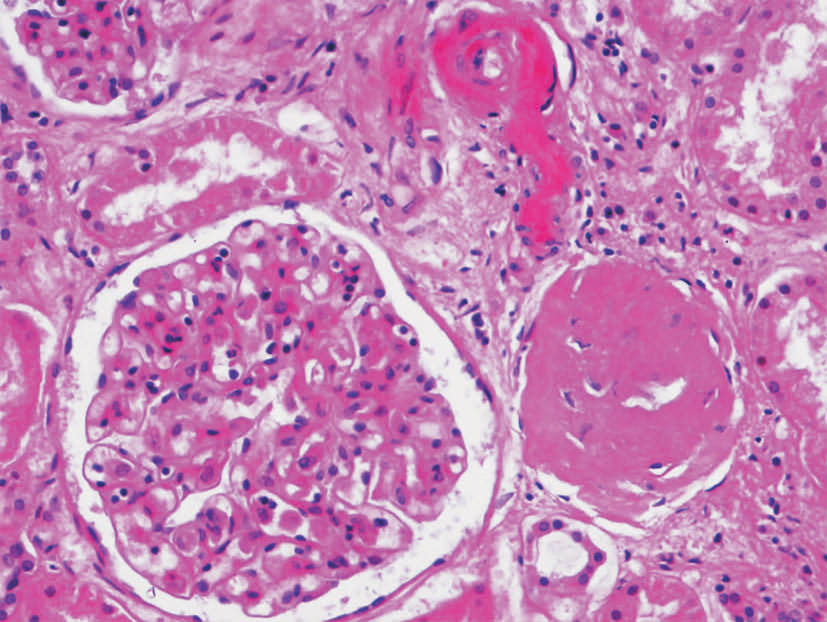
\includegraphics{./images/Image00100.jpg}
    \captionsetup{justification=centering}
    \caption{细动脉硬化肾(HE染色,中倍)\\{\small 图中可见细动脉玻璃样变,病变严重的肾小球发生纤维化、玻璃样变,所属肾小管萎缩、消失,间质纤维化,健存肾小球代偿性肥大}}
    \label{fig6-8}
\end{figure}



(3)脑:由于脑细小动脉的痉挛和硬化,患者脑部可出现一系列病变,主要有脑水肿、脑软化和脑出血。

1)脑水肿:由于脑内细小动脉的硬化和痉挛,局部组织缺血,毛细血管通透性增加,以致发生脑水肿,严重时临床表现以脑病的症状与体征为特点,病人剧烈头痛,呕吐、意识障碍、精神错乱,甚至昏迷、局灶性或全身性抽搐,称为高血压脑病。

2)脑软化(softening of
brain):脑细小动脉硬化伴有痉挛时,局部脑组织缺血、坏死,出现多数小坏死灶,即微梗死灶。常发生于壳核、尾状核、丘脑、桥脑、小脑等处,其他部位较少见。光镜下见梗死灶脑组织液化坏死,形成质地疏松的筛网状病灶。由于软化灶较小,一般不引起严重后果。软化灶的坏死组织逐渐吸收,由胶质细胞增生修复。

3)脑出血(cerebral
hemorrhage):脑出血是高血压病最重要的并发症,也是最常见的死因。出血多见于内囊、基底节,其次为大脑白质、桥脑和小脑。出血灶内脑组织完全被破坏,形成囊腔,其内充满坏死的脑组织和凝血块。出血范围大时,可破入侧脑室(图\ref{fig6-9})。高血压脑出血的原因可归纳为三种情况:①当脑内小动脉痉挛时,局部脑组织缺血、缺氧,细小动脉通透性增加,同时管腔内血液的压力高,而引起漏出性出血。②高血压病人脑细小动脉本身变硬变脆或血管壁弹性减弱向外膨出形成微小动脉瘤,当血压突然升高时,血管壁或微小动脉瘤可破裂出血。③大脑出血多发生在基底节、丘脑和内囊部,是因为供应该区域的豆纹动脉从大脑中动脉呈直角分支,而且比较细,受大脑中动脉压力较高的血流直接冲击和牵引,易使已有病变的豆纹动脉破裂出血。脑出血的后果主要取决于出血的量和出血部位。较大量出血时,病人常突然发生昏迷、呼吸加深,脉搏加快,出现陈-施呼吸、瞳孔反射及肌腱反射消失、大小便失禁等症状和体征。内囊部出血时,可引起对侧肢体偏瘫及感觉消失。出血破入侧脑室时,患者发生昏迷,常导致死亡。左侧脑出血常引起失语。脑桥出血可引起同侧面瘫及对侧肢体偏瘫。

\begin{figure}[!htbp]
    \centering
    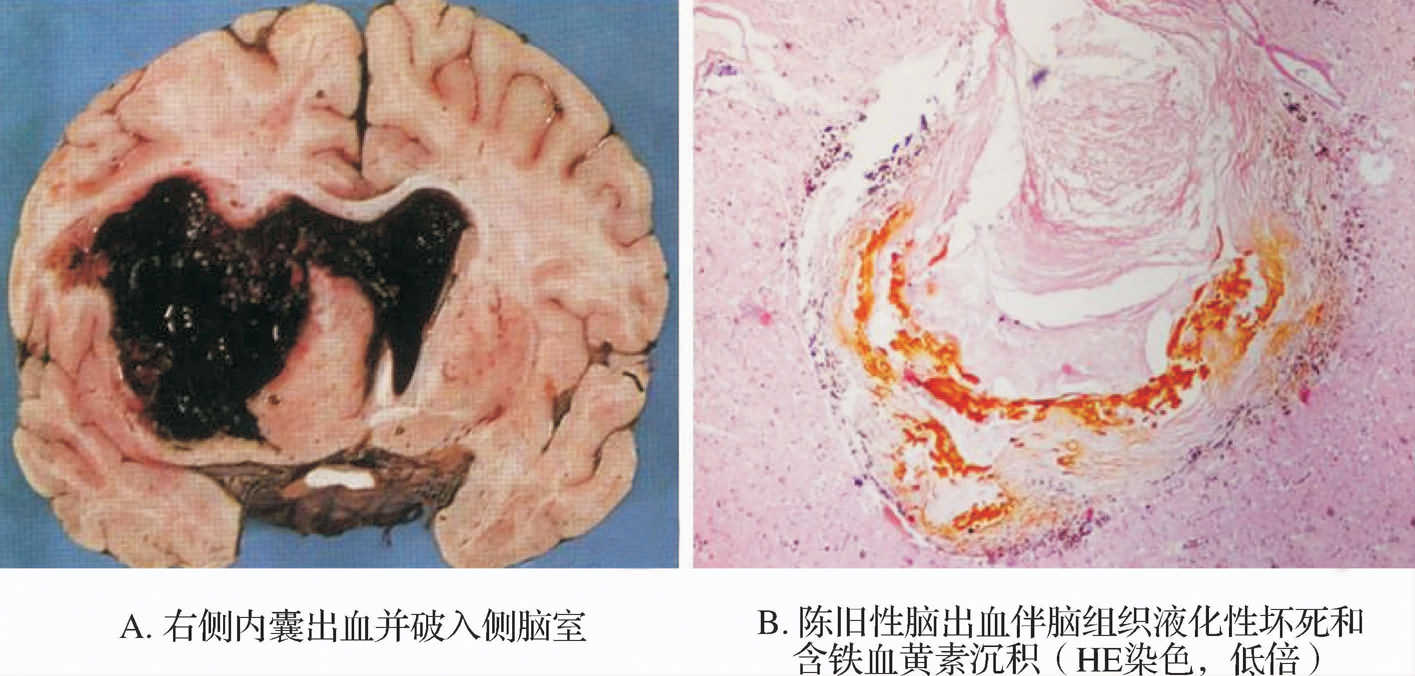
\includegraphics{./images/Image00101.jpg}
    \captionsetup{justification=centering}
    \caption{高血压性脑出血}
    \label{fig6-9}
\end{figure}

\paragraph{视网膜}
眼底镜检查表现为:病变早期视网膜中央动脉痉挛;中期血管迂曲,变细而苍白,反光增强,有动、静脉交叉压迫现象;晚期或严重者视乳头发生水肿,视网膜渗出和出血,患者视物模糊。

\subsubsection{恶性高血压病(malignant hypertension)}

恶性高血压病又称急进型高血压。本型较少见,可由良性高血压病恶化而来,也可起病即为急进型。病理上以细、小动脉管壁的纤维素样坏死和增生性小动脉内膜炎为特征。全身各器官血管均可受累,但以肾小球入球动脉和脑的细小动脉病变尤为严重。在肾脏,细、小动脉病变还常并发血栓形成,可引起出血及微梗死。脑的血管病变常造成局部缺血、微梗死和脑出血。

临床上,患者多为青少年,血压显著升高,舒张压常持续在17.3~18.6
kPa(130~140
mmHg)或更高。可发生高血压脑病,常有持续的蛋白尿、血尿和管型尿。本病病程短、预后差,多数患者于1年内死于尿毒症,也可因脑出血或心力衰竭而死亡。

\section{风湿病}
\begin{framed}
    {案例6-3}

    {【病例摘要】}

    有一病人曾患游走性四肢大关节炎数年,近半年来心悸、气短,近一个月两下肢水肿,查体颈静脉怒张,肝大肋缘下3
    cm,二尖瓣听诊可闻及双期杂音。

    {【问题】}

    (1)本患者的疾病正确诊断应为什么?

    (2)试分析其心脏可能出现的病理变化及形成机制。
\end{framed}

风湿病(rheumatism)是一种与A组β溶血性链球菌感染有关的变态反应性炎性疾病。病变可累及全身结缔组织,表现为胶原纤维的变性、坏死,继而出现细胞增生,形成具有诊断特征的风湿肉芽肿。本病常侵犯心脏和关节,其次为皮肤、浆膜、脑和血管等,其中以心脏病变最为严重。本病急性期称为风湿热(rheumatic
fever),临床上常出现反复发作的心肌炎、多发性关节炎、皮肤环形红斑、皮下结节和小舞蹈症等,并伴有发热、血沉加快和抗链球菌溶血素O抗体滴度增高等表现。多次反复发作后,常造成轻重不等的心瓣膜器质性病变。

风湿病是一种常见病,在我国东北和华北地区发病率高,冬春季多见。本病可发生于任何年龄,但多始发于5~14岁,女性多于男性。

\subsection{病因和发病机制}

风湿病的发生与A组β溶血性链球菌感染有关。大多数病人发病前2~3周有链球菌性咽峡炎、扁桃体炎史,95%病人血中抗链球菌溶血素O(ASO)、抗链球菌激酶等抗体的滴度升高,及时的抗生素治疗和预防链球菌感染可预防风湿病的初发或复发,但风湿病的本质为无菌性、非化脓性炎症,提示本病并非链球菌本身直接引起。风湿病的发病机制尚未完全明了,目前多数倾向于抗原抗体交叉反应学说。A组β溶血性链球菌细胞壁上C抗原(糖蛋白)和M蛋白与机体结缔组织中的某些成分具有共同抗原性,因此,链球菌感染后机体产生的抗体不仅作用于细菌,也与自体结缔组织成分起交叉免疫反应,导致风湿病的发生。也有人认为链球菌感染可能激发患者对自身抗原的自身免疫反应,而引起相应病变。

\subsection{基本病变}

风湿病可侵犯全身结缔组织,病变发展过程大致可分为三期。

\paragraph{变质渗出期}
开始是结缔组织纤维发生黏液样变性,胶原纤维肿胀,基质内蛋白多糖增多。以后肿胀的胶原纤维断裂,崩解成红染无结构的颗粒状物,即纤维素样坏死。此时,病灶内可有少量浆液和炎性细胞(淋巴细胞,少量中性白细胞和单核细胞)浸润。此期持续约1个月。

\paragraph{增生期}
亦称肉芽肿期,其特点是形成对本病具有诊断意义的风湿肉芽肿,即风湿小体,或称阿少夫小体(Aschoff
body)。风湿小体多见于心肌间质,心内膜下和皮下结缔组织。风湿小体多为球形、椭圆形或梭形,其中心常为纤维素样坏死,周围有一定数量的风湿细胞(Aschoff
cell),外围有少量淋巴细胞和单核细胞(图\ref{fig6-10})。风湿细胞的形态特点是细胞体积较大呈圆形或多边形,胞浆丰富,嗜碱性。核大,常为圆形或卵圆形,空泡状,核膜清楚,有时为多个核。染色质集中于核的中央并呈细丝状向核膜发散,横切面上状似枭眼,纵切面上形如毛虫。关于风湿细胞的来源尚有争议,但现代标记技术证明其为巨噬细胞源性。此期可持续2~3个月。

\begin{figure}[!htbp]
    \centering
    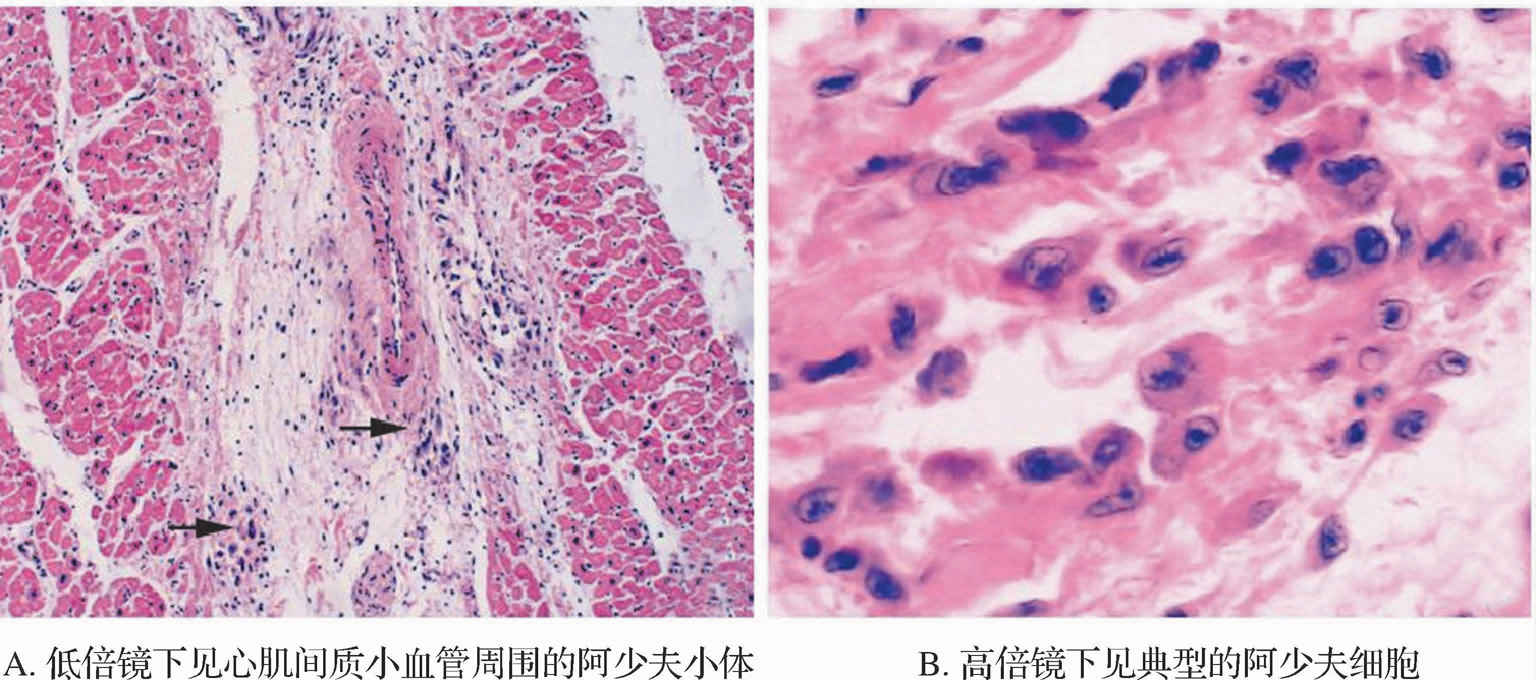
\includegraphics{./images/Image00102.jpg}
    \captionsetup{justification=centering}
    \caption{风湿性心肌炎(HE染色)}
    \label{fig6-10}
\end{figure}

\paragraph{瘢痕期或愈合期}
此期风湿小体内的纤维素样坏死物被溶解吸收,风湿细胞转变为成纤维细胞,产生胶原纤维,风湿小体逐步变为梭形小瘢痕。此期可持续2~3个月。

上述3期改变的自然经过为4~6个月,但因风湿病可反复发作,故不同时期的病变常同时并存。病变持续反复进展,可致严重的纤维化和瘢痕形成。

\subsection{风湿性心脏病}

风湿病时,病变累及心脏引起风湿性心脏病(rheumatic heart
disease)。初次发作的风湿热患者中,约35%可累及心脏,表现为风湿性心内膜炎、风湿性心肌炎和风湿性心外膜炎。如各层均受累,则称为风湿性全心炎。风湿性心内膜炎发生在所有风湿性心脏病的病人,而风湿性心肌炎和风湿性心外膜炎仅发生在严重病例。

\subsubsection{风湿性心内膜炎}

风湿性心内膜炎(rheumatic
endocarditis)病变主要侵犯心瓣膜,其中以二尖瓣最常受累,其次是二尖瓣和主动脉瓣同时受累,三尖瓣和肺动脉瓣极少受累。也可累及瓣膜邻近的心内膜和腱索。病变早期,瓣膜结缔组织发生黏液样变性、纤维素样坏死、浆液渗出和炎细胞浸润,偶见风湿小体,导致瓣膜肿胀增厚。病变瓣膜表面,尤以闭锁缘向血流面的内皮细胞,由于受到瓣膜开关时的摩擦而受损脱落,暴露其下胶原,血小板和纤维素在该处沉积,形成单行排列的,直径为1~2
mm大小的灰白色、半透明、疣状赘生物,为白色血栓,其紧密附着于瓣膜,不易脱落(图\ref{fig6-11})。

\begin{figure}[!htbp]
    \centering
    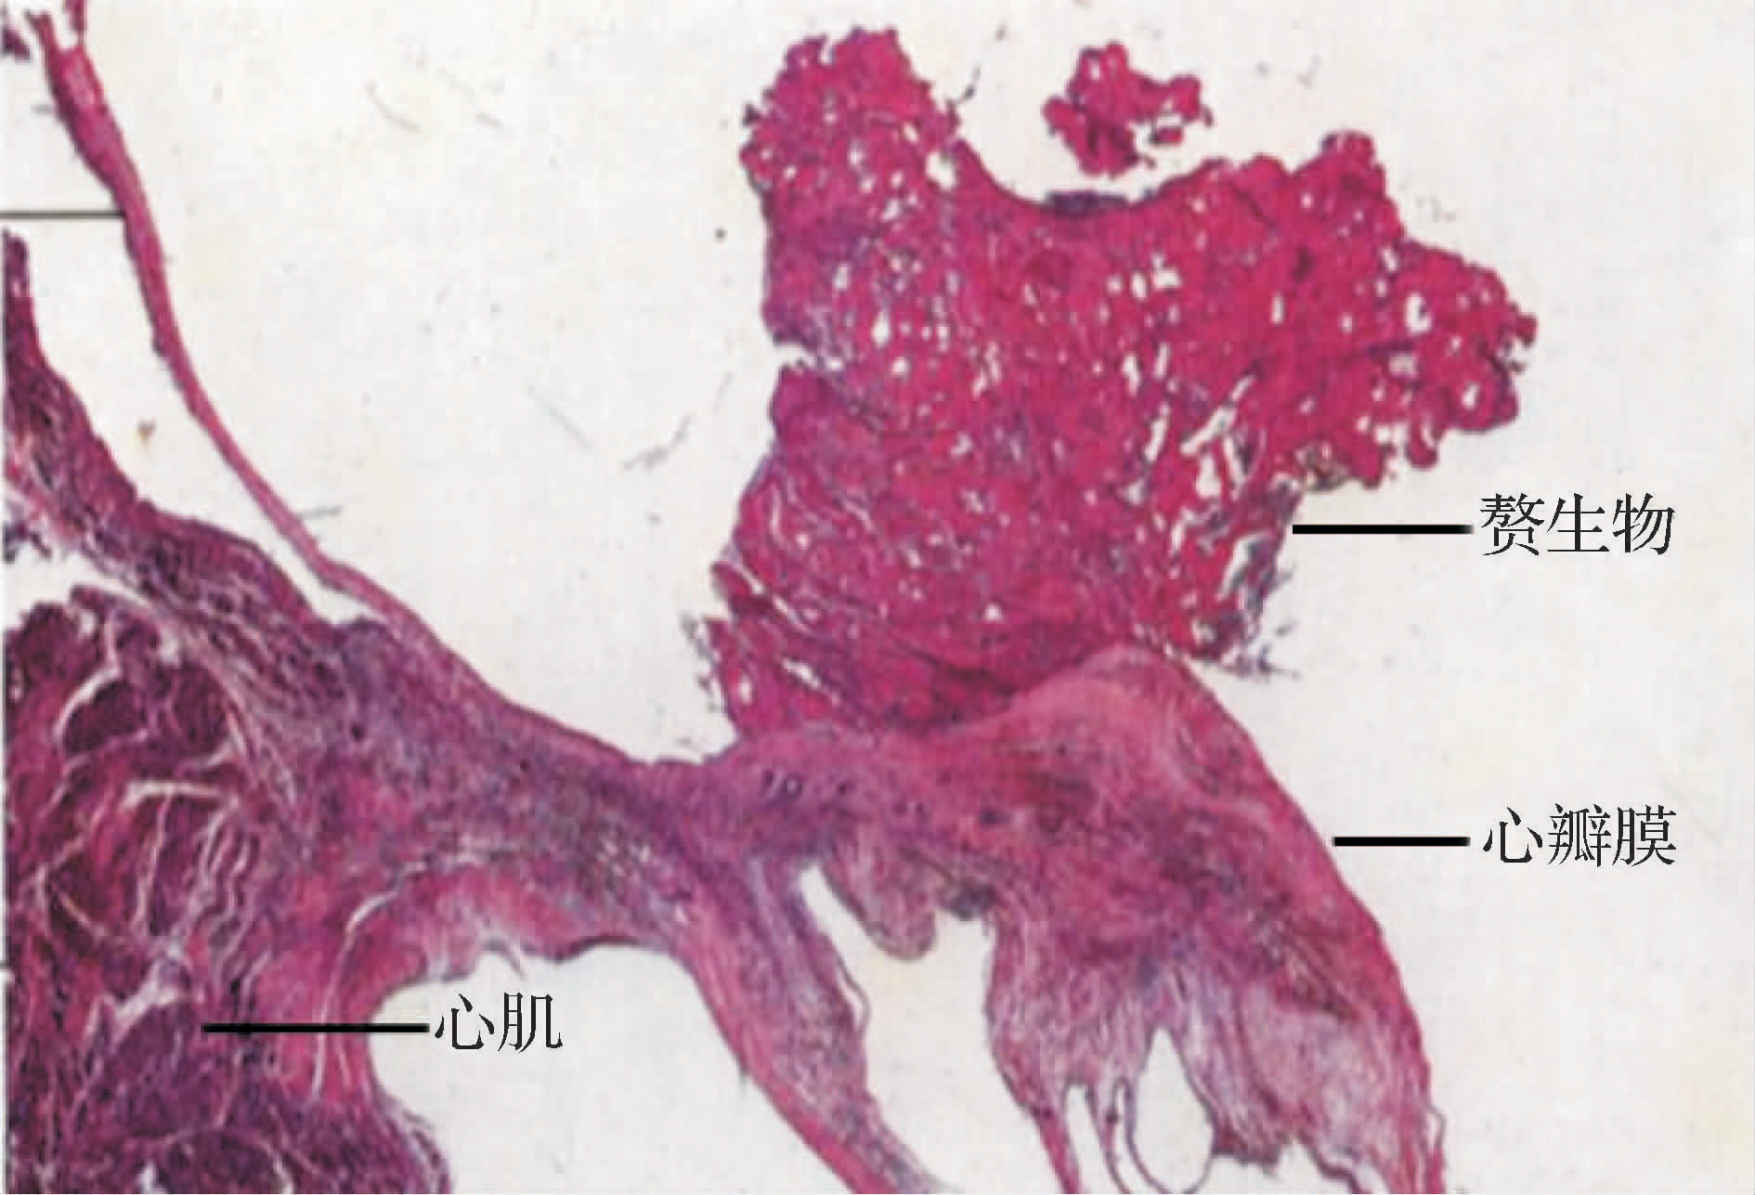
\includegraphics{./images/Image00103.jpg}
    \captionsetup{justification=centering}
    \caption{风湿性心内膜炎(HE染色,低倍)\\{\small 图中可见增厚的心瓣膜以及附着的赘生物}}
    \label{fig6-11}
\end{figure}



由于病变反复发作和不断机化,导致结缔组织增生,使瓣膜增厚、变硬、卷曲、缩短,瓣叶间粘连以及腱索增粗和缩短,最终形成慢性风湿性心瓣膜病。

\subsubsection{风湿性心肌炎}

风湿性心肌炎(rheumatic
myocarditis)主要累及心肌间质结缔组织,病变特征是在心肌间质小血管附近出现风湿小体。后期,风湿小体发生纤维化,形成梭形小瘢痕。此病变最常见于左心室后壁、室间隔以及左心室后乳头肌等处。发生于儿童者,有时渗出性病变特别明显,心肌间质明显水肿,有较多的淋巴细胞、嗜酸性粒细胞甚至中性粒细胞浸润。病变较轻的病人,可无明显症状,如病变较重而广泛,则可影响心肌收缩力,表现为心率加快,第一心音低钝,如病变波及传导系统,可发生传导阻滞,儿童患者可发生心功能不全。

\subsubsection{风湿性心外膜炎(心包炎)}

风湿性心外膜炎(rheumatic
pericarditis)的病变主要累及心包脏层,呈浆液性或浆液纤维素性炎症。心包腔内可有大量浆液性渗出物,引起心包积液,叩诊时心界向左、右扩大,听诊时心音遥远。当大量纤维素渗出时,由于心包的脏层和壁层不断摩擦,使心外膜表面的纤维素形成绒毛状,称为绒毛心。恢复期,渗出的浆液和纤维素逐渐被吸收。若纤维素吸收不完全,则发生机化,造成心包脏层和壁层之间部分粘连,极少数病例心包腔可完全闭锁,形成缩窄性心包炎,影响心脏的搏动,进而发生心功能不全。

\subsection{心脏外的风湿病变}

\subsubsection{风湿性关节炎}

约75%的风湿热病人早期出现风湿性关节炎(rheumatic
arthritis)。病变常累及大关节,如膝、踝、肩、腕及肘关节等,病变呈多发性、游走性,各关节常先后受累,反复发作。关节局部组织出现红、肿、热、痛和活动受限等炎症表现。病变主要为关节滑膜的浆液性炎,滑膜及关节周围组织充血、水肿,胶原纤维黏液样变性和纤维素样坏死,有时可见不典型风湿小体形成。愈复后,浆液性渗出物被完全吸收,一般不留后遗症。

\subsubsection{风湿性动脉炎}

风湿性动脉炎可发生于冠状动脉、肾动脉、肠系膜动脉、脑动脉、主动脉和肺动脉等处,大小动脉均可受累,以小动脉受累较为常见。急性期主要病变是血管壁的黏液样变性和纤维素样坏死,伴淋巴细胞浸润,可有风湿小体形成。后期因瘢痕形成而使管壁呈不规则增厚,可导致管腔狭窄。

\subsubsection{皮肤病变}

\paragraph{环形红斑(erythema marginatum)}
是风湿病急性期发生于皮肤的渗出性病变,常见于躯干和四肢皮肤。对急性风湿病具有诊断意义。病变为环形淡红色斑,边缘红,中央色泽正常,1~2日可自行消退。光镜下见红斑处真皮浅层血管充血,周围水肿伴淋巴细胞和单核细胞浸润。

\paragraph{皮下结节(subcutaneous nodules)}
是以增生为主的皮肤病变。一般见于大关节附近伸侧面皮下,直径为0.5~2
cm,圆形或椭圆形,质地较硬,可以活动,压之不痛。光镜下,结节中心有纤维素样坏死物质,周围可见纤维母细胞和风湿细胞围绕呈栅栏状排列,伴淋巴细胞浸润。数周后,结节逐渐纤维化而形成瘢痕。风湿热时,皮下结节并不经常出现,一旦出现,具有诊断价值。

\subsubsection{中枢神经系统病变}

多见于儿童,女孩居多。主要病变为风湿性脑动脉炎,可出现神经细胞变性,胶质细胞增生。病变以大脑皮质、基底节、丘脑和小脑皮层最明显。当锥体外系统病变严重时,患儿常出现肢体的不自主运动,称为小舞蹈症(chorea
minor)。

\section{感染性心内膜炎}

感染性心内膜炎(infective
endocarditis)是指由病原微生物直接侵袭心内膜,尤其是心瓣膜而引起的内膜炎症,其特征病变为心瓣膜表面形成含有病原微生物的赘生物,常伴有败血症和栓塞现象。引起心内膜炎的因素有:①病原体侵入血流,引起菌血症、败血症等,并侵袭心内膜。常见病原体包括各种细菌、真菌、病毒等;②心瓣膜损伤,有利于病原微生物寄居繁殖;③防御机能的抑制,如应用免疫抑制剂后。感染性心内膜炎可按临床经过和病变特点分为亚急性和急性两类。

\subsection{亚急性感染性心内膜炎}

亚急性感染性心内膜炎大多由毒力较弱的细菌感染引起,尤以草绿色链球菌最常见(约占75%),少数由其他链球菌、肠球菌、葡萄球菌、淋球菌、真菌(白色念珠菌)等引起。病程经过6周以上,可迁延数月甚至1~2年。病原菌多从机体内某一感染灶(如扁桃体炎、牙周炎、骨髓炎等)侵入血流;亦可因拔牙、心导管和心脏手术等医源性感染侵入血流,引起败血症,并侵犯心内膜。此型心内膜炎常发生于已有病变的瓣膜上,50%~80%发生在风湿性心内膜炎的基础上,或并发于先天性心脏病(如室间隔缺损等)。常常侵犯二尖瓣和主动脉瓣,并可累及其他部位心内膜。

\subsubsection{病理变化}

肉眼观:可见在原有病变的瓣膜上形成赘生物。二尖瓣和主动脉瓣病变最为常见而严重,瓣膜呈不同程度增厚、变形,其表面可见大小不一的赘生物(图\ref{fig6-12}A)。赘生物为灰黄色,干燥而质脆,易脱落,瓣膜可以出现溃疡,一般较急性者为浅,但亦可发生穿孔。光镜下:赘生物主要为混合血栓,由血小板、纤维素、细菌菌落、炎性细胞和少量坏死组织构成,细菌菌落常包裹于血栓内部(图\ref{fig6-12}B)。瓣膜溃疡底部可见不同程度的肉芽组织增生和淋巴细胞、单核细胞及少量中性白细胞浸润,有时还可见到原有风湿性心内膜炎的病变。

\begin{figure}[!htbp]
    \centering
    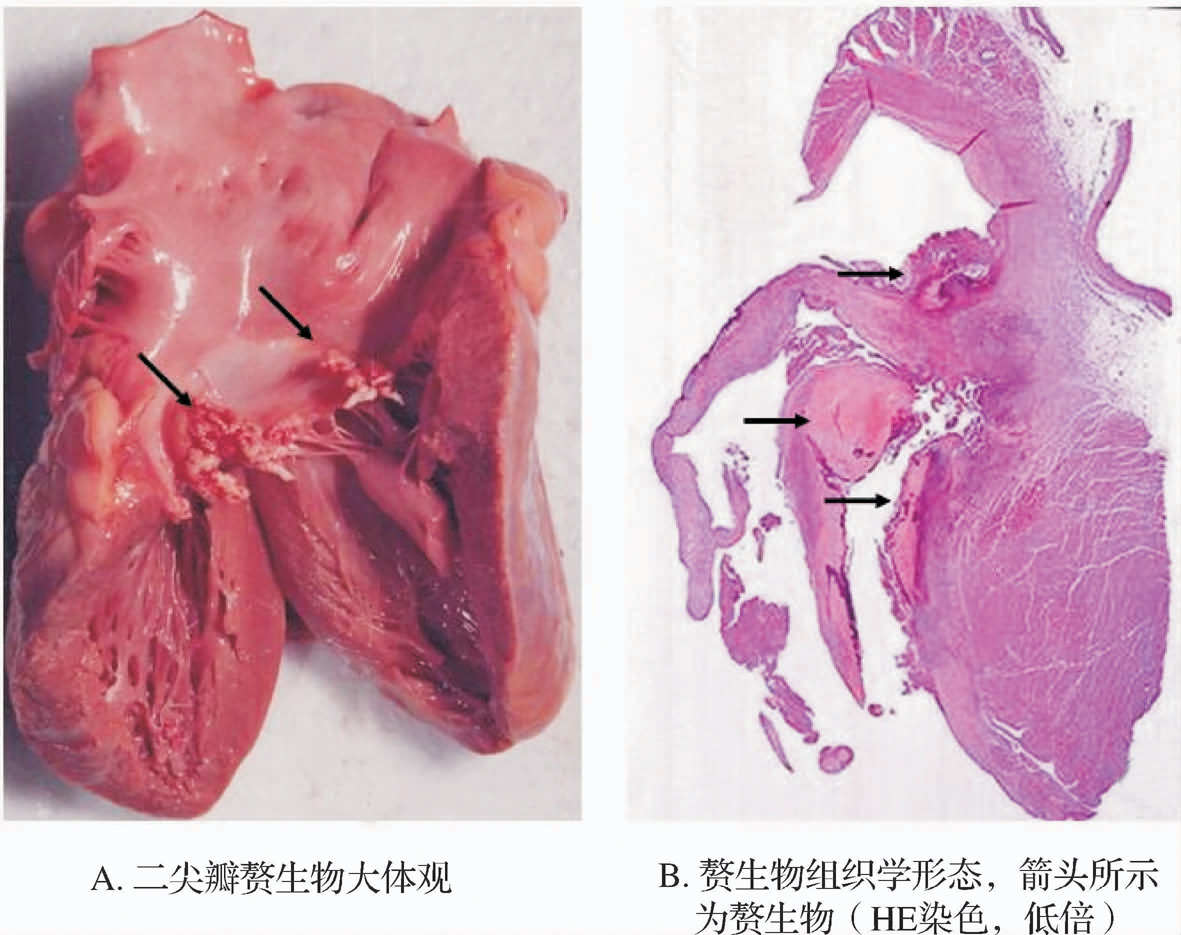
\includegraphics{./images/Image00104.jpg}
    \captionsetup{justification=centering}
    \caption{亚急性感染性心内膜炎之瓣膜赘生物}
    \label{fig6-12}
\end{figure}

\subsubsection{临床病理联系}

临床上,可闻及心脏杂音且杂音强度和性质常呈多变性,后者是由于赘生物的变化(增大、破碎或脱落等)所致。赘生物内的细菌侵入血流,引起败血症,患者可出现脾肿大、贫血、皮肤黏膜出血点。脾一般中度肿大,与毒素刺激单核巨噬细胞系统增生及脾窦充血有关;由于细菌的轻度溶血作用以及脾功能亢进,常引起患者贫血;患者皮肤、黏膜和眼底常有出血点,这是由于血管壁受损,通透性升高所致。此外,由于瓣膜上的赘生物松脆,容易脱落形成栓子,因而临床上常出现脑、肾及脾动脉栓塞和梗死。有时皮下出现红色有压痛的结节(称为Osler结节),其发生可能与免疫复合物性脉管炎有关。可因微栓塞或抗原抗体复合物的作用引起肾小球肾炎。

亚急性感染性心内膜炎的治愈率较高,但愈后的瘢痕造成严重的瓣膜变形和腱索增粗缩短,导致瓣口狭窄和(或)关闭不全。少数病例可因急性瓣膜功能不全,或因心、脑等重要器官的栓塞或严重的败血症而危及生命。

\subsection{急性感染性心内膜炎}

急性感染性心内膜炎常为全身严重化脓菌感染引起的重要并发症,多由毒力较强的化脓菌引起,其中大多为金黄色葡萄球菌。通常病原菌先在某局部引起化脓性炎症(如痈、化脓性骨髓炎等),当机体抵抗力降低时病菌侵入血流,引起败血症并侵犯心内膜。此型心内膜炎多发生在原本正常的心内膜上,常单独侵犯主动脉瓣或二尖瓣,引起急性化脓性心内膜炎。

\subsubsection{病理变化}

病变瓣膜溃烂、严重者可发生瓣膜破裂穿孔,腱索断裂。在病变瓣膜表面形成赘生物,主要由脓性渗出物、混合血栓、坏死组织和大量细菌混合而成。细菌分布于赘生物表面和内部。这些赘生物一般较大,灰黄或浅绿色,质地松软,易脱落形成感染性栓子(图\ref{fig6-13})。

\begin{figure}[!htbp]
    \centering
    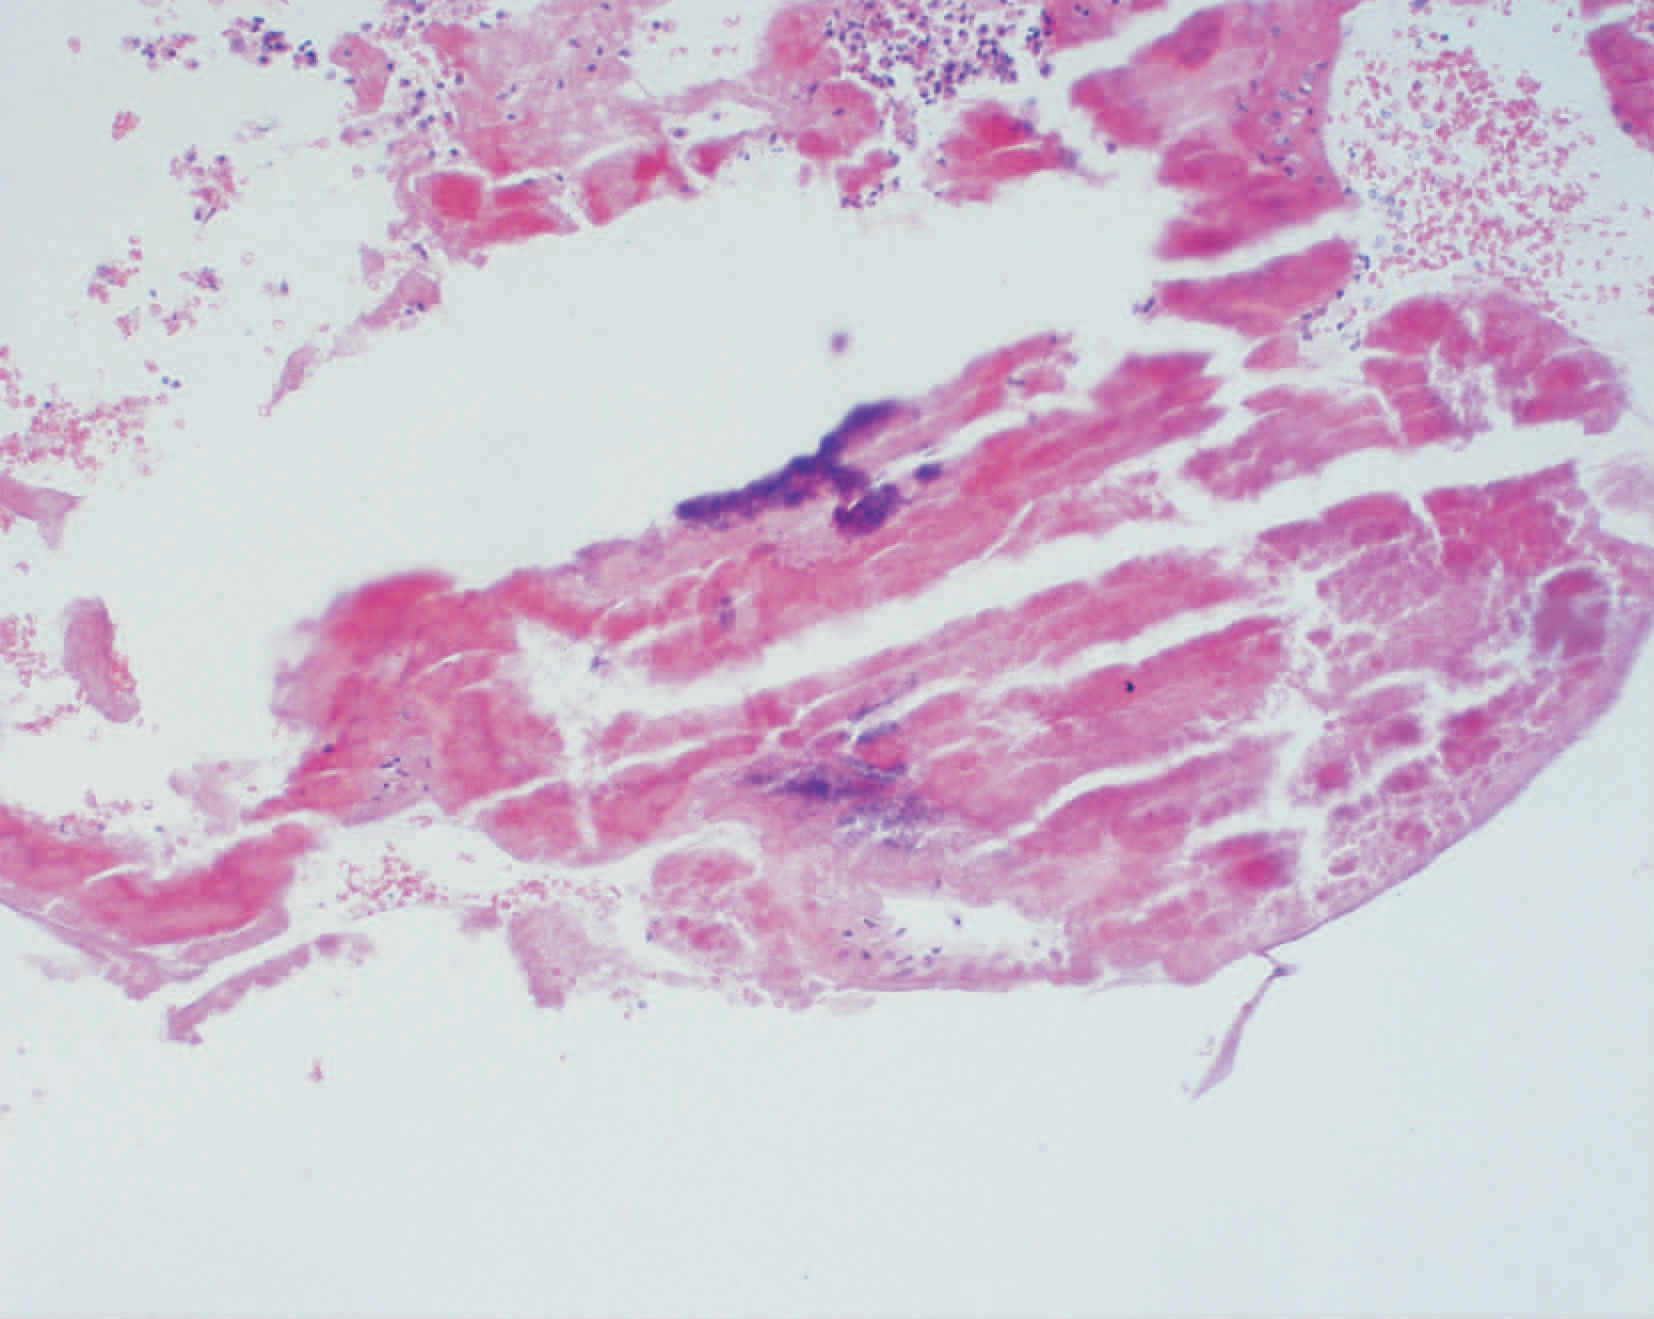
\includegraphics{./images/Image00105.jpg}
    \captionsetup{justification=centering}
    \caption{急性细菌性心内膜炎(HE染色,低倍)\\{\small 心瓣膜上的赘生物。血栓中混有多量的细菌菌落}}
    \label{fig6-13}
\end{figure}



\subsubsection{结局和并发症}

急性感染性心内膜炎时,由于含菌赘生物易于脱落,引起栓塞,常造成体循环一些器官的梗死和多发性栓塞性小脓肿。瓣膜破裂、穿孔或腱索断裂,可导致急性心瓣膜关闭不全而猝死。由于抗生素的广泛使用,死亡率已大大下降,但受损的瓣膜经瘢痕修复后常导致严重的慢性心瓣膜病。

\begin{table}
    \centering
    \caption{各种心内膜炎的比较}
    \label{tab6-1}
    \begin{tabular}{lp{4cm}p{4cm}p{4cm}}
        \toprule
        名称                                                                                               & 风湿性心内膜炎                                                                   & 亚急性感染性心内膜炎                                                 & 急性感染性心内膜炎                         \\
        \midrule
        病因                                                                                               & A族乙型链球菌感染有关的变态反应                                                  & 草绿色链球菌直接感染心瓣膜                                           & 毒力强的化脓性细菌直接感染心瓣膜
        \\
        好发部位                                                                                           & 二尖瓣、二尖瓣和主动脉瓣的闭锁缘                                                 & 二尖瓣、主动脉瓣游离缘                                               & 主动脉瓣、二尖瓣游离缘
        \\
        病理变化                                                                                           & 赘生物细小串珠状排列,质地坚硬,不易脱落;镜下主要为血小板和纤维素构成的白色血栓 &
        赘生物较大,质软,息肉状,单个或多个,易脱落;镜下混合血栓内含有炎症细胞、细菌菌落及少许坏死组织等 &
        赘生物最大,质脆,极易脱落,受累瓣膜常穿孔、溃疡;镜下混合血栓内可见大量中性粒细胞、细菌、 坏死组织等                                                                                                                                                                                                     \\
        结局                                                                                               & 多次反复发作引起各种瓣膜病,导致心力衰竭                                         & 赘生物脱落导致栓塞、梗死,并加重瓣膜疾病。可因心衰、梗死、败血症死亡 & 赘生物脱落导致栓塞性脓肿,多因脓毒血症死亡 \\
        \bottomrule
    \end{tabular}
\end{table}

\section{心瓣膜病}

心瓣膜病(valvular diseases of the
heart)是指心瓣膜因先天性发育异常或后天疾病造成的器质性病变,表现为瓣膜口狭窄(valvular
stenosis)和(或)关闭不全(valvular
insufficiency),常导致心功能不全,引起全身血液循环障碍。心瓣膜病大多为风湿性心内膜炎反复发作的结果,感染性心内膜炎、主动脉粥样硬化和梅毒性主动脉炎等亦可引起。瓣膜口狭窄和关闭不全可单独发生,但通常两者合并存在(瓣膜双病变)。最常见于二尖瓣,其次是主动脉瓣。病变可累及一个瓣膜,或两个以上瓣膜同时或先后受累(联合瓣膜病)。

瓣膜口狭窄是指瓣膜口开放时不能充分张开,造成血流通过障碍。常由于相邻瓣膜之间互相粘连,瓣膜增厚,弹力减弱或瓣环硬化、缩窄等引起。

瓣膜关闭不全是指心瓣膜关闭时不能完全闭合,使一部分血液发生反流,通常是由于瓣膜增厚、变硬、卷曲、缩短,或由于瓣膜破裂和穿孔而引起。

\subsection{二尖瓣狭窄}

二尖瓣狭窄(mitral
stenosis)主要是由于风湿性心内膜炎反复发作,二尖瓣瓣膜交界处粘连、增厚、变硬或钙化所致。正常成人二尖瓣口面积约为5
cm$^2$ ,可以通过两个手指。狭窄时,瓣膜口面积不同程度缩小。

\subsubsection{分型}

按病变程度可将二尖瓣狭窄分为3型:①隔膜型:病变最轻,瓣膜仅轻度增厚,主要是瓣膜边缘粘连。②增厚型:除瓣膜间粘连外,瓣膜明显增厚,瓣口狭窄较重。③漏斗型:瓣膜极度增厚,瓣口形如漏斗或鱼口状,极度狭窄,瓣膜口面积可缩致1~2
cm$^2$,甚至0.5 cm$^2$ ,常伴关闭不全(图\ref{fig6-14}A)。

\subsubsection{血流动力学改变和心脏变化}

早期,由于二尖瓣口狭窄,舒张期从左心房注入左心室的血液受阻,舒张末期仍有部分血液滞留于左心房内,加上由肺静脉回流的血液,致左心房血量比正常增多,因而左心房发生代偿性扩张,左心房心肌加大收缩力以克服狭窄瓣膜口的阻力把血液排入左心室,久之导致左心房代偿性肥大。后期,左心房代偿失调,心房收缩力减弱,最终左心房高度扩张(肌原性扩张)、淤血。左心房内血液淤积致肺静脉回流受阻,引起肺淤血、肺水肿或漏出性出血。由于肺静脉压力升高,通过神经反射引起肺内小动脉收缩,使肺动脉压升高,长期肺动脉高压可导致右心室代偿肥大,失代偿时,发生肌原性扩张,当右心室高度扩张时,右心室瓣膜环随之扩大,出现三尖瓣相对关闭不全,收缩期右心室部分血液返回右心房,继而右心房淤血、扩张,最后导致右心功能不全,引起体循环淤血。

心脏的变化表现为“三大一小”,因流入左心室的血量减少,左心室无明显变化甚至缩小,而左心房、右心房和右心室均肥大扩张。

\subsubsection{临床病理联系}

二尖瓣狭窄听诊时在心尖区可闻及隆隆样舒张期杂音。这是由于舒张期左心房血液经过狭窄的二尖瓣口注入左心室时形成涡流所致。X线检查,显示左心房明显增大,呈“梨形”心影。由于左心衰竭导致肺淤血、水肿及漏出性出血,患者常咳出粉红色泡沫痰,出现呼吸困难、发疳等。右心衰竭时,体循环淤血,出现颈静脉怒张,肝淤血肿大,下肢水肿,浆膜腔积液。

\subsection{二尖瓣关闭不全}

二尖瓣关闭不全(mitral
insufficiency)的病因以风湿性心内膜炎最多见,其次为感染性心内膜炎。

由于二尖瓣关闭不全,心脏收缩时左心室的部分血液返流到左心房,加上肺静脉回流的血液,致左心房肥大和扩张。当心脏舒张时,左心房将多于正常量的血液排入左心室,使左心室因负荷增加而发生肥大和扩张(图\ref{fig6-14}B)。在左心房和左心室代偿失调发生左心衰竭后,依次引起肺淤血、肺动脉高压、右心室和右心房代偿性肥大、右心衰竭及体循环淤血。

\begin{figure}[!htbp]
    \centering
    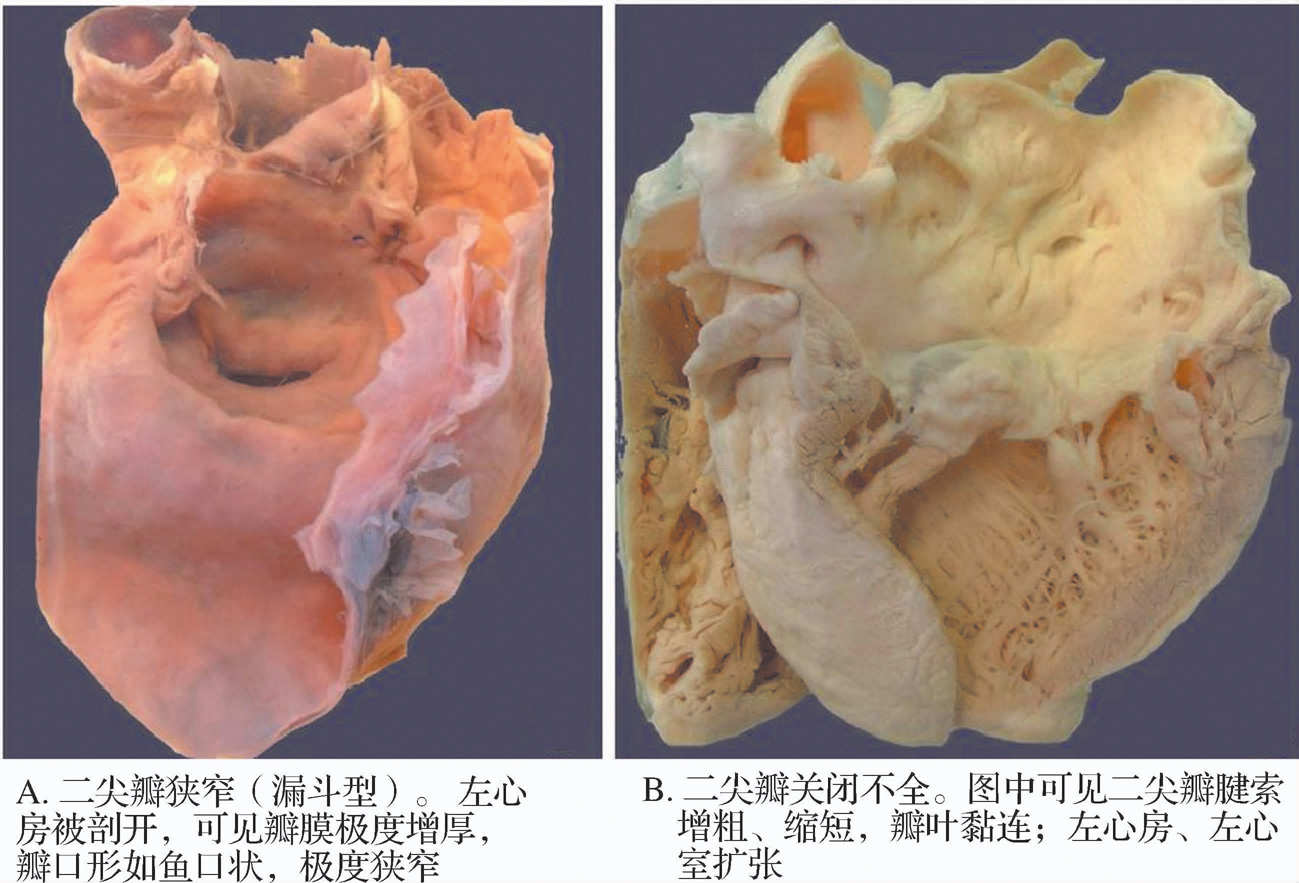
\includegraphics{./images/Image00107.jpg}
    \captionsetup{justification=centering}
    \caption{心瓣膜病}
    \label{fig6-14}
\end{figure}

二尖瓣关闭不全患者心尖区可闻及吹风样收缩期杂音。X线检查见左心室肥大,全心衰竭时,左右心房、心室均肥大扩张,呈“球形”心影。

\subsection{主动脉瓣狭窄}

主动脉瓣狭窄(aortic
stenosis)比较少见,主要是慢性风湿性主动脉瓣膜炎的后果,常与二尖瓣病变合并发生。由于瓣膜口狭窄,在心脏收缩期,左心室血液排出受阻,发生代偿性肥大,左室壁肥厚,但心腔不扩张(向心性肥大)。由于左心室代偿能力强,代偿期可长达数年不出现左心衰竭的表现。后期,左心室代偿失调而发生肌原性扩张,左心室血量增多,继之出现左心房淤血、肺淤血、肺动脉高压、右心肥大、右心衰竭和体循环淤血。

主动脉瓣狭窄的患者在主动脉瓣听诊区可闻及收缩期喷射性杂音。严重狭窄者,心输出量极度减少,血压降低,内脏,特别是冠状动脉供血不足,可产生心绞痛。

\subsection{主动脉瓣关闭不全}

主动脉瓣关闭不全(aortic
insufficiency)主要由风湿性主动脉瓣膜炎造成。此外也可因主动脉粥样硬化和梅毒性主动脉炎累及主动脉瓣膜所致。由于瓣膜口关闭不全,在心脏舒张期,主动脉部分血液返流入左心室,使左心室因血容量增多而逐渐发生代偿性肥大。久之,代偿失调发生肌原性扩张,依次引起左心房肥大扩张、肺淤血、肺动脉高压、右心肥大、右心衰竭和体循环淤血。

听诊时,在主动脉瓣区可闻及舒张期杂音。由于舒张期主动脉部分血液反流,舒张压下降,故脉压差增大。患者可出现水冲脉、血管枪击音及毛细血管搏动现象。由于舒张压降低,冠状动脉供血不足,有时可出现心绞痛。

\section{心肌炎和心肌病}

\subsection{心肌炎}

心肌炎(myocarditis)是由各种原因引起的心肌的局限性或弥漫性炎症。心肌炎的发病率逐年增高,因而该病日益受到重视。引起心肌炎的病因很多,可以是生物性的致病因素,如病毒、细菌、螺旋体、真菌和寄生虫感染等;可以是免疫性因素,如伴发于某些变态反应性疾病或与某些药物过敏有关;可以是物理或化学的损害或中毒引起;另有部分心肌炎的原因不清楚,如孤立性心肌炎。

\subsubsection{病毒性心肌炎}

病毒性心肌炎(viral
myocarditis)绝大多数是由亲心肌的病毒感染引起。可引起心肌炎的病毒很多,其中以柯萨奇病毒B组感染最为常见,ECHO病毒、流感病毒、风疹病毒等引起的也较为多见。病变的特点为心肌间质非特异性炎症。早期心肌细胞灶性变性坏死,间质淋巴细胞和中性白细胞浸润;以后出现巨噬细胞聚集和纤维组织增生;最后形成心肌间质纤维化,可伴有代偿性心脏肥大。少数病例病变严重,大片心肌坏死,病人可死于心搏骤停。病变可以累及传导系统,造成心律异常,出现相应的临床表现和心电图改变。

\subsubsection{细菌性心肌炎}

细菌性心肌炎(bacterial
myocarditis)通常是由化脓菌直接感染引起的心肌炎症。常见的致病菌有金黄色葡萄球菌、溶血性链球菌、肺炎双球菌。病变常作为全身脓毒败血症的一个部分,化脓菌来源于感染灶或细菌性心内膜炎时含有细菌的栓子。病变肉眼观,心脏表面及切面可见多发性灰黄色小脓肿灶,周围有充血出血带。光镜下,可见典型的化脓性炎症改变,灶性心肌细胞坏死液化,脓细胞集聚,可见细菌集落。脓肿周围心肌有不同程度的变性、坏死及间质中性粒细胞和单核巨噬细胞浸润。

\subsubsection{孤立性心肌炎}

孤立性心肌炎(isolated
myocarditis)又称为Fiedler心肌炎,原因不明,好发生于中、青年人。急性型常伴有心力衰竭、心脏扩张,可猝死。依据组织学变化分为两型。

\paragraph{弥漫性间质性心肌炎}
心肌细胞较少发生变性、坏死,心肌间质小血管周围有多量淋巴细胞、浆细胞和巨噬细胞浸润,也可以出现多少不一的嗜酸性粒细胞和中性白细胞浸润。

\paragraph{特发性巨细胞性心肌炎}
心肌细胞局灶性坏死及肉芽肿形成。病灶中央坏死,呈红染、无结构状,周围有淋巴细胞、浆细胞、单核巨噬细胞和嗜酸性粒细胞浸润,并混有较多大小不一的多核巨细胞,表现为异物型或Langhans型多核巨细胞。

\subsection{心肌病}

心肌病(cardiomyopathy)是指伴有心肌功能障碍的心肌疾病。1995年世界卫生组织和国际心脏病学会工作组根据病理生理学、病因学和发病因素将心肌病分为四型,包括扩张性心肌病、肥厚性心肌病、限制性心肌病和致心律失常性右心心肌病。

\subsubsection{扩张性心肌病}

扩张性心肌病(dilated
cardiomyopathy)又称充血性心肌病,是以进行性心肌肥大、心腔扩张和心肌收缩能力下降为特征。主要病变为心脏体积增大,重量增加,可达500~800
g甚至更重。各心腔均明显扩张,心室壁略增厚或正常(心肌肥厚为明显扩张的心腔所掩盖),心尖部变薄呈钝圆形,常见附壁血栓形成。心脏苍白色,心内膜增厚及纤维化。光镜下,心肌细胞不均匀性肥大、伸长,核大、深染及畸形。肥大和萎缩的心肌细胞交错排列。心肌细胞常发生空泡变、小灶性肌溶解、微小坏死灶或小瘢痕灶。

临床上常表现为进行性心力衰竭,部分病人可发生猝死。

\subsubsection{肥厚性心肌病}

肥厚性心肌病(hypertrophic
cardiomyopathy)特点是心肌肥大、室间隔不对称肥厚、使心室腔显著缩小,舒张期充盈异常及左心室流出道受阻,以流出道梗阻明显与否分为梗阻性和非梗阻性肥厚性心肌病。肉眼观:心脏增大,重量增加,成人常达500
g以上,两侧心室肌肥厚,尤以室间隔肥厚为明显,呈球形隆起。光镜下:心肌纤维高度肥大,排列紊乱,走向各异或呈漩涡状(图\ref{fig6-15})。

\begin{figure}[!htbp]
    \centering
    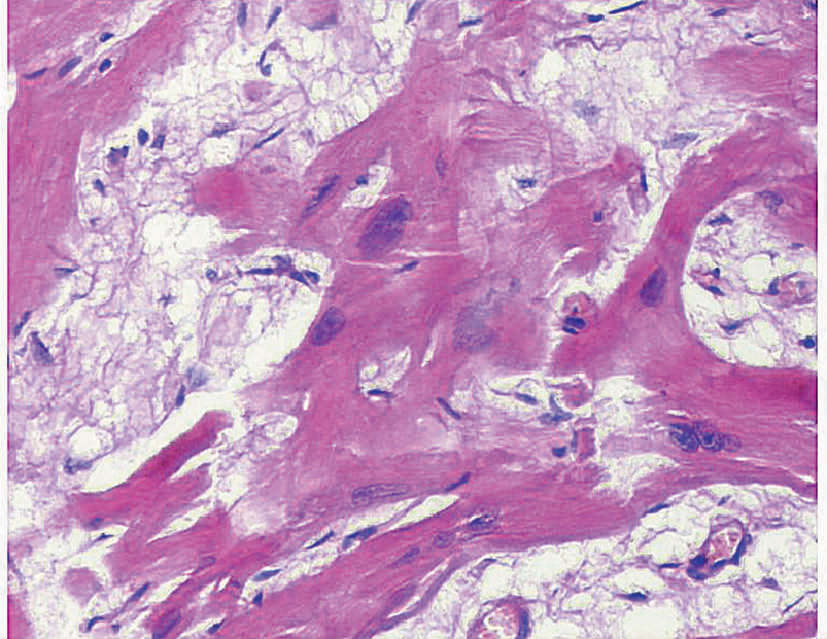
\includegraphics{./images/Image00108.jpg}
    \captionsetup{justification=centering}
    \caption{肥厚性心肌病(HE染色,高倍)\\{\small 镜下见心肌纤维高度肥大,排列紊乱}}
    \label{fig6-15}
\end{figure}



临床上部分患者可无自觉症状,而因猝死或在体检中被发现。许多患者有心悸、胸痛或在劳累后出现气急,伴有流出道梗阻的患者由于左心室充盈不足,心排血量减低可在起立或运动时出现眩晕,甚至神志丧失。

\subsubsection{限制性心肌病}

限制性心肌病(restrictive
cardiomyopathy)以单侧或双侧心室充盈受限和舒张期容量降低为特点,典型病变为心室内膜和内膜下心肌进行性纤维化并有附壁血栓形成,引起心室壁僵硬和部分心腔阻塞。临床上主要表现为心力衰竭和栓塞,少数可发生猝死。

\subsubsection{致心律失常性右室心肌病}

致心律失常性右室心肌病(arrhythmogenic right ventricular
cardiomyopathy)又称右室心肌病,特征为右心室心肌被纤维脂肪组织进行性替代(图\ref{fig6-16}),早期呈区域性,逐渐可累及整个右心室甚至部分左心室。临床常表现为心律失常、右心扩大和猝死,尤其在年轻患者。

\begin{figure}[!htbp]
    \centering
    
\includegraphics{./images/Image00109.jpg}
    \captionsetup{justification=centering}
    \caption{致心律失常性右室心肌病(HE染色,低倍)\\{\small 右心室心肌萎缩,脂肪组织增生替代}}
    \label{fig6-16}
\end{figure}



\section*{复习与思考}

{一、名词解释}

风湿小体 风湿细胞 小舞蹈病 向心性肥厚 高血压性固缩肾 动脉瘤 室壁瘤 Osler结节 粥瘤

{二、问答题}

1. 试述动脉粥样硬化症的基本病理变化。

2. 试述动脉粥样斑块各种复合病变的形成及危害。

3. 试述心肌梗死的常见部位、病变特点及并发症。

4. 良、恶性高血压的基本病理改变有什么异同?

5. 试述良性高血压内脏病变期心、脑、肾和视网膜的主要病理变化。

6. 风湿病的基本病变是什么?风湿病对人体的主要危害是什么?

7. 比较二尖瓣狭窄与关闭不全时血流动力学改变和相应心脏病变的异同点。

8.
试列表比较风湿性心内膜炎与细菌性心内膜炎(从病因、发病部位、病变特点及结局等方面比较)。

{三、临床病理分析}

病史摘要:患者男性,58岁,某单位保卫人员。于某夜间骑自行车巡逻时突然死亡。其家人称,死者生前嗜烟酒,曾有过“心口痛”病史。其他病史不详。

尸检所见:死者身长170 cm,较肥胖。

主动脉:主动脉全长可见内膜多处黄白色斑块,并伴有溃疡及钙化;镜下见主动脉内膜纤维组织增生,内膜下为多量坏死崩解的无定形物及胆固醇结晶,病灶处钙化。

冠状动脉:左冠状动脉前降支质硬如电线,以起始段为重。切面见管腔阻塞超过3/4。

心脏:重380
g,左心室前壁心肌软,土黄色,灰暗无光泽,病变达心肌全层。左心室前壁近心尖处破裂,破裂口长约1.5
cm。心包腔内积血约500 ml。

镜下见左心室壁心肌呈凝固性坏死。

双肾:体积缩小,各为115
g,表面颗粒状,并可见扩张的小囊泡,切面皮质约厚0.2 cm。

镜下见双肾弥漫性细小动脉硬化,管壁增厚、腔小。肾小球玻璃样变,肾小管萎缩,肾间质纤维组织增生,炎细胞浸润。残存肾单位代偿性肥大。

脑:脑内小血管周围可见含铁血黄素沉着。

讨论题:

1. 试述本病例的病理诊断和诊断依据。

2. 试述本病的发生发展过程以及主要病变间的相互关系。

3. 本例死亡原因是什么?